%%%%(c)
%%%%(c)  This file is a portion of the source for the textbook
%%%%(c)
%%%%(c)    Abstract Algebra: Theory and Applications
%%%%(c)    Copyright 1997 by Thomas W. Judson
%%%%(c)
%%%%(c)  See the file COPYING.txt for copying conditions
%%%%(c)
%%%%(c)
%In the last chapter we introduced a new notation for functions called tableau notation.

%\begin{exercise}
%Suppose for instance that $f : U \to V$, where $U = \{1, 2, 3, 4, 5, 6\}$, $V = \{ A, B, C, D, E, F\}$, and $f = \{(1,C), (2,B), (3,D), (4,A), (5,E), (6,F)\}$.  
%\begin{enumerate}[(a)]
%\item
%Write $f$ in tableau form.
%\item
%Is $f$ a symmetry?  Explain why or why not.
%\end{enumerate}
%\end{exercise} 

%This function is a bit different from the functions we dealt with in the Symmetries chapter, specifically because its domain and range aren't the same.  But the tableau notation can be used to represent this function just the same.  In fact, 

%\begin{exercise}
%Suppose that $g : U \to W$, where $U = \{1, 2, 3, 4, 5, 6\}$, $W = \{ M, N, O, P\}$, and $f = \{(1,P), (2,M), (3,O), (4,N), (5,M), (6,P)\}$.
%\begin{enumerate}[(a)]
%\item
%Write $g$ in tableau form.
%\end{enumerate}
%\end{exercise}

%Here the number of elements, or cardinality, of the domain and range don't even match; but nonetheless the ableau notation can be used.

%In practice however, tableau notation is seen and used most often for functions like those we saw in the Symmetries chapter:  bijections whose domain and codomain are the same.  These functions are given a specific name -- Permutations.

\chap{Permutations}{permute}

\begin{quote}
"For the real environment is altogether too big, too complex, and too fleeting for direct acquaintance. We are not equipped to deal with so much subtlety, so much variety, so many permutations and combinations. And although we have to act in that environment, we have to reconstruct it on a simpler model before we can manage it." 
\medskip

\noindent (Source: Walter Lippmann, Pulitzer prize-winning journalist)
\end{quote}

We mentioned at the beginning of  the ``Functions'' chapter that we would be interested in functions on finite sets. In this chapter we will investigate the gory details of one-to-one onto functions whose domain and range are the same finite set. Until now we have looked at functions as  mappings that take set elements to other set elements. In this chapter, we will begin to consider functions as elements in their own right. This new point of view will culminate in the realization that \emph{all} finite groups are in some sense groups of functions (if you don't understand this yet, don't worry--you will by the end of the chapter).
\footnote{Thanks to Tom Judson for material used in this chapter.}

\section{Introduction to permutations}

In Chapter~\ref{symmetries} we saw that all symmetries are  bijections whose domain and codomain were the same.  Thus symmetries are special cases of \emph{permutations}, which are defined mathematically as follows.

\begin{defn}
A bijection whose domain and codomain are equal is called a \bfii{ permutation}\index{Permutation!definition of}\index{Bijection!as a permutation}. The set of all bijections from a finite set $X$ to itself is called the \bfii{ set of permutations on $X$} and is denoted as $S_X$.
\end{defn}

\begin{example}
Let us recall for a moment the equilateral triangle $\bigtriangleup ABC$ from the Symmetries chapter.  
%%\## reference
Let $T$ be the set of vertices of $\bigtriangleup ABC$; i.e. $T = \{ A, B, C \}$.  We may list the permutations of $T$ as follows.  For input $A$, we have 3 possible outputs; then for $B$ we would have two possible outputs (to keep the one-to-one property of each combination); and finally for $C$ only one possible output.  Therefore there are $3 \cdot 2 \cdot 1 = 6$ permutations of $T$.  Below are the six permutations in  $S_T$:
 
\begin{gather*}
\begin{pmatrix}
A & B & C \\
A & B & C
\end{pmatrix}
\qquad
\begin{pmatrix}
A & B & C \\
C & A & B
\end{pmatrix}
\qquad
\begin{pmatrix}
A & B & C \\
B & C & A
\end{pmatrix}
\\
\begin{pmatrix}
A & B & C \\
A & C & B
\end{pmatrix}
\qquad
\begin{pmatrix}
A & B & C \\
C & B & A
\end{pmatrix}
\qquad
\begin{pmatrix}
A & B & C \\
B & A & C
\end{pmatrix}
\end{gather*}
\end{example}

\noindent
Which of these permutations are symmetries of the equilateral triangle?  
%% give reference.
%Look back at Figure~\ref{groups_s3_symmetry_fig} in the Symmetries chapter. 
In the Symmetries chapter we saw that they all are: so in this case the set of symmetries on $T$ is equal to $S_T$.

Now suppose instead we label the vertices of an \emph{isosceles} triangle as $A, B, C$, and let $T$ represent these vertices.  In this case,  $S_T$  is the same as before: it doesn't matter what arrangement or position the vertices are in, or even if $A$, $B$, and $C$ are vertices at all.  The permutations depend only on the set $T$, and are oblivious to whether or not they correspond to the vertices of some figure.
 
But what about the symmetries of an isosceles triangle? It turns out that an isosceles triangle has only two symmetries (see exercise below). 
So  the set of symmetries on $T$ is a subset of $S_T$, but not the whole set.

\begin{exercise}\label{exercise:permute:isos_tri_sym}
Suppose that the two congruent sides of triangle $ABC$ are $\overline{AB}$ and $\overline{BC}$). Give the two symmetries, in tableau form.
\end{exercise}

\begin{exercise}\label{exercise:permute:tri_sym}
Suppose $T$ is used to represent any three-sided figure.  
%\begin{enumerate}[(a)]
%\item
Which permutation(s) does the set of symmetries of $T$ always contain?
%% CPT I don't understand the following item
%\item
%Because of (a), for all figures that can be represented by $T$, what can we conclude about the set of symmetries of those %figures (compared to $S_T$)?
%\end{enumerate}
\end{exercise}

\begin{exercise}\label{exercise:permute:S_4}
Suppose $X = \{A, B, C, D\}$.
\begin{enumerate}[(a)]
\item
How many permutations are there on $X$?
\item
List $S_X$.
\item
List the elements in $S_X$ that are not symmetries of the square.
\item
What additional elements in $S_X$ are not symmetries of the rectangle?
\end{enumerate}
\end{exercise}

In fact, it's obvious to see that \emph{any} symmetry is a permutation, since a symmetry is by definition a bijection from a finite set of points to itself.  But as we've seen in Exercises~\ref{exercise:permute:isos_tri_sym}, ~\ref{exercise:permute:tri_sym}, ~\ref{exercise:permute:S_4} (as well as Exercise~\ref{exercise:symmetries:bijectnotsym} from the Symmetries chapter), \emph{not} all permutations (bijections) correspond to a symmetry.  Given a set $X$ then that represents a figure, the set of symmetries from $X \to X$ is a subset of $S_X$.


\section{Permutation groups and other generalizations}

%Suppose in the exercise above that $X = \{1, 2, 3, 4\}$ instead of $\{A, B, C, D\}$.  Could we still represent a four-sided figure with $X$.  Of course; we can label the vertices of the figure whatever we want.  More importantly, 

We saw in the Symmetries chapter that the set of symmetries of any figure form a group under the operation of function composition. Since we've already seen that permutations are closely related to symmetries, this naturally leads to the question:  is $S_X$ a group under function composition?  Fortunately, this time the answer is easier to prove.
%Given a set $X$ with $n$ elements, we could represent any n-sided figure with $X$.  Let's say $Y = \{\mbox{ symmetries of %the n-sided figure }\}$.  Then from above we know $Y \subset S_X$.  And from the Symmetries chapter we know $Y$ is a group under function composition (do you remember why?).  Hence the elements of $Y$ are a group under function %composition; the elements of $Y$ also happen to be elements of $S_X$; and in fact all the elements of $S_X$ are functions, particularly bijections.  Curiosity then leads us to the question:  is $S_X$ a group under function composition?  

\begin{prop}\label{proposition:permute:S_X_group}
Given any set $X$, $S_X$ is a group under function composition.\index{Composition!of symmetries}
\end{prop}

\begin{proof}
\begin{itemize}
\item
First then, if $f, g \in S_X$, then $f \compose g$ would be, by definition of composition, a function from $X \to X$.  Further, since it is a composition of two bijections, $f \compose g$ would be a bijection (proved in Functions chapter).  Therefore by definition $f \compose g$ is permutation from $X \to X$.  In other words $f \compose g \in S_X$.  So $S_X$ is closed under function composition.\index{Composition!of permutations}
\item
Second, the identity of $S_X$ is just the permutation that sends every element of $X$ to itself (We will call this permutation ${\var id}$, just like we did with symmetries.)\index{Permutation!identity}\index{Identity!of a permutation}.  
\item
Third, if $f \in S_X$, then by definition $f$ is a bijection; hence from the Inverse section of the Functions chapter we know $f$ has an inverse $f^{-1}$ from $X \to X$ that is also a bijection.  Hence $f^{-1} \in S_X$.  Therefore every permutation in $S_X$ has an inverse.\index{Permutation!inverse}\index{Inverse!of permutations} 
\item
Finally, composition of functions is associative, which makes the group operation associative.  
\end{itemize}

Hence $S_X$ is a group under function composition.
\end{proof}

\subsection{The symmetric group of $n$ letters}

We can label the vertices of a triangle as $A, B, C$ or $1, 2, 3$ or $\var{apple, pear, cherry}$ or whatever, without changing the triangle. No matter how we label the triangle, the symmetries of the triangle will be the "same" in some sense (although we write them down differently). 

Since symmetries are special cases of permutations, this motivates us to investigate the effect of relabeling on permutations in general.

For starters, we'll look at a simple example. Let $X = \{A, B, C, D\}$ and $Y = \{1, 2, 3, 4\}$.  Suppose 

\begin{center}
$\mu = \begin{pmatrix} A & B & C & D\\ D & C & B & A \end{pmatrix}$, $\sigma = \begin{pmatrix} A & B & C & D\\ C & D & A & B \end{pmatrix}$ 

\medskip
and 

$\tau = \begin{pmatrix} 1 & 2 & 3 & 4\\ 4 & 3 & 2 & 1 \end{pmatrix}$, $\rho = \begin{pmatrix} 1 & 2 & 3 & 4\\ 3 & 4 & 1 & 2 \end{pmatrix}$ \\ 
\end{center}

\noindent
Is $\mu = \tau$?  Technically no,  because they their domain/codomains are different, yet we can clearly see that they are somehow equivalent.  But how do we express this equivalence?

Suppose we start with the tableau for $\mu$. We cross out every `A' in the tableau and replace with `1'. Similarly, we replace $B, C, D$ with $2, 3,4$ respectively. Then what we end up with is exactly $\tau$.  In other words, performing a ``face-lift''  on $\mu$ gives $\tau$.  Therefore $\mu$ and $\tau$ are equivalent, as are $\sigma$ and $\rho$.  

\begin{exercise}\label{exercise:permute:7}
\begin{enumerate}[(a)]
\item
Write $\mu \compose \sigma$ in tableau form.
\item
Write $\tau \compose \rho$ in tableau form.
\item
Is $ \mu \compose \sigma$ equivalent to $\tau \compose \rho$? \emph{Explain} your answer.
\item
Is $\sigma \compose \mu$ equivalent to $\rho \compose \tau$?  \emph{Explain} your answer.
\end{enumerate}
\end{exercise}

Let's summarize our findings so far:
\begin{itemize}
\item
The \emph{sets} $S_X$ and $S_Y$ are equivalent in the following sense: for each element of $S_X$ we can find an equivalent element of $S_Y$ by replacing $A, B, C, D$ with $1, 2, 3, 4$.  

\item
Further, as we saw in the exercises,  the composition of two elements in $S_X$ is equivalent to the composition of the two equivalent elements in $S_Y$.  So we can say that composition acts the ``same'' on both sets.
\end{itemize}


So far we have only looked at sets with four elements. Now it's time to generalize these results to sets of any size. First, some notation:

\begin{notation}{}
The \bfii{ order of a set} $Y$ is the number of elements of $Y$, and is written as $|Y|$.\index{Order! of a set}
\footnote{ You're probably used to seeing $|\ldots|$ as representing absolute value. Of course a set is not a number, so it has no absolute value. We use $|Y|$ to denote order because it's a measure of the \emph{size} of set $Y$, just as the absolute value of a number is the ``size'' of the number.}
\end{notation}

Now let $X = \{1,2,\ldots, n\}$, and  consider any set $Y$ with $|Y| = n$. We could do a similar ``face-lifting'' as above to show that  $S_X \equiv S_Y$.  So the group $S_X$ is equivalent to the permutations of \emph{any} set of $n$ elements.

\begin{notation}{sym_group_n_letters}
Let $X=\{ 1, 2, \ldots, n\}$. Instead of writing $S_X$, we write $S_n$\label{symmetricgroup}.  $S_n$ is called the \bfii{ symmetric group\index{Group!symmetric} on $n$ letters}.
\end{notation}

\subsection{Isomorphic groups}

At the end of the Symmetries chapter, we compared the groups $\mathbb{Z}_n$, the $n$ rotations of a regular n-gon, and the $n^{th}$ roots of unity.  We saw that, as long as you made a suitable pairing (bijection) between the elements of any two of these sets, then their Cayley tables were exactly the same. 

We've just seen the very same thing for $S_n$. The above statement that ``the composition of two elements in $S_X$ is equivalent to the composition of the two equivalent elements in $S_Y$''  is the same thing as saying that  the Cayley table entries are equivalent between the two groups.

This "equivalence of groups" is one of the premier concepts in abstract algebra, almost as important as the concept of a group  itself.  When two groups are equivalent like this, we say that they are \bfii{ isomorphic groups}; we also say that the bijection that causes the groups to be equivalent is an \bfii{ isomorphism}\index{Isomorphic groups}\index{Group!isomorphic}\index{Isomorphism!definition of}.  We will see in a later chapter how to show in general that two groups are isomorphic; but for now, forming the groups' Cayley Tables and seeing if you can match elements to make the tables the same is a very good strategy.

\begin{exercise}
Let $W =\{G, H \}$ and $Z = \{J, K \}$.
\begin{enumerate}[(a)]
\item
Write the Cayley Tables for $S_W$ and $S_Z$. It would be helpful to write the entries of $S_W$ and $S_Z$ in tableau form. 
\item
Give a bijection from $W$ to $Z$, and the corresponding bijection from $S_W$ to $S_Z$, that would show $S_W$ is isomorphic to $S_Z$. (Remember that a bijection can be thought of as  a ``relabeling'' of elements of $W$ as elements of $Z$.)
\item
*How many possible bijections from $W$ to $Z$ give rise to isomorphisms from  $S_W$ to  $S_Z$?
\end{enumerate}
\end{exercise}


\begin{exercise}\label{exercise:permute:11}
Let $X =\{A, B, C\}$ and $Y = \{M, N, P\}$.
\begin{enumerate}[(a)]
\item
Write the Cayley Tables for $S_X$ and $S_Y$
\item
Give a bijection from $X$ to $Y$, and the corresponding bijection from $S_X$ to $S_Y$, that would show $S_X$ is isomorphic to $S_Y$.
\item
*How many possible bijections from $X$ to $Y$ produce isomorphisms from $S_X$ to $S_Y$?
\item
*Now let $X =\{A, B, \ldots M\}$ and $Y = \{N, O, \ldots Z\}$. How many different bijections from $X$ to $Y$ produce isomorphsims from $S_X$ to $S_Y$?

\end{enumerate}
\end{exercise}

\subsection{Subgroups and permutation groups}

Let's summarize this section so far.  The permutations on a set $X$ of $n$ elements is a group under function composition (denoted by  $S_n$).  Further, for any figure with $n$ sides, the symmetries of that figure is a subset of $S_n$ containing at least the identity permutation, and that subset is itself a group under function composition.  This example motivates the following definition.

\begin{defn}
A subset of a group $G$ that is itself a group under the same operation as $G$ is called a \bfii{ subgroup}\index{Subgroup} of $G$.  
\end{defn}

The notion of subgroup is a key concept in abstract algebra, which will be used throughout the rest of the book.  

\begin{example}\label{example:permute:subgroups}
From the above definition of subgroup it follows that:
\begin{itemize}
\item
The symmetries of a rectangle are a subgroup of $S_4$. 
\item
The symmetries of an isosceles triangle are a subgroup of $S_3$.
\item
$D_5$ is a subgroup of $S_5$.
\item
The permutations of $\{1,2,3\}$ are a subgroup of the permutations of $\{1,2,3,4\}$. Hence $S_3$ is a subgroup of $S_4$. By the same token, $S_m$ can be considered as a subgroup of $S_n$ whenever $m < n$.
\end{itemize}
\end{example}

%Now, let us generalize again.  Suppose we were looking at the set of symmetries for a rectangle.  We've proved it's a group by the properties of symmetries and bijections.  If we took that set of permutations and "erased" the rectangle, would the permutations still be a group?  If the set didn't correspond to the symmetries of a figure, would the permutations sill act as a group?  They should, because whether the permutation are connected to a figure or not, they should still act the same when you compose them.  In fact it makes sense that they would, because the Cayley Table for that set of permutations would remain exactly the same.  Therefore you would still have closure under function composition, and the operation of the identity permutation and existence of inverses would remain exactly the same.  The associativity of the set wouldn't change, because function composition is still associative.  Nothing would actually change.  So the permutations that correspond to the symmetries of a rectangle are a subgroup in their own right.  This leads to the following generalization and definition:

\begin{defn}
A subgroup of $S_n$ is called a \bfii{ permutation group}\index{Group!permutation}\index{Permutation group}.
\end{defn}

\begin{exercise}\label{exercise:permute:permute_S5}
Consider the subset $G$ of $S_5$ consisting of the identity
permutation ${\var id}$ and the permutations 
\begin{align*}
\sigma
& =
\begin{pmatrix}
1 & 2 & 3 & 4 & 5 \\
1 & 2 & 3 & 5 & 4
\end{pmatrix} \\
\tau
& =
\begin{pmatrix}
1 & 2 & 3 & 4 & 5 \\
3 & 2 & 1 & 4 & 5
\end{pmatrix} \\
\mu
& =
\begin{pmatrix}
1 & 2 & 3 & 4 & 5 \\
3 & 2 & 1 & 5 & 4
\end{pmatrix}.
\end{align*}
\begin{enumerate}[(a)]
\item
Write the Cayley table for $G$ (Label your rows and columns as: ${\var id}, \sigma, \tau, \mu$).
\item
Use the Cayley table to explain whether $G$ is a subgroup of $S_5$ or not.  

\medskip
\emph{Remember: you don't need to show the associative property, since function composition is associative.}
\end{enumerate}
\end{exercise}

\begin{exercise}\label{exercise:permute:permute_S4}
Consider the subset $G$ of $S_4$ consisting of the identity
permutation ${\var id}$ and the permutations 
\begin{align*}
\sigma
& =
\begin{pmatrix}
1 & 2 & 3 & 4  \\
2 & 3 & 1 & 4
\end{pmatrix} \\
\tau
& =
\begin{pmatrix}
1 & 2 & 3 & 4  \\
3 & 2 & 1 & 4 
\end{pmatrix} \\
\mu
& =
\begin{pmatrix}
1 & 2 & 3 & 4  \\
3 & 1 & 2 & 4 
\end{pmatrix}.
\end{align*}
\begin{enumerate}[(a)]
\item
Write the Cayley table for $G$ (Label your rows and columns as: ${\var id}, \sigma, \tau, \mu$).
\item
Use the Cayley table to explain whether or not $G$ is a subgroup of $S_4$.
\end{enumerate}
\end{exercise}

As the example shows, a permutation group need not comprise all symmetries of a figure or all rearrangements of a set. Many permutation groups have no evident practical interpretation whatsoever. Nonetheless they are still useful, because as we shall see they can be used to characterize the groups that contain them.
 
% So whether the permutations of $G$ correspond to any physical phenomena or not, $G$ is a permutation group.  This may not seem amazing, but as we'll see in coming chapters, knowing all possible subgroups of a group goes a long way to figuring out the structure and properties of that group, even to determining sometimes if two groups are isomorphic.  And subgroups aren't always going to correspond to actual phenomena.  In fact in the next section we'll discover a couple more permutation groups that have virtually no correspondence to real-world phenomena, but nonetheless we can prove are groups.


%I was going to use this here, but I will use it as the introduction to the Groups chapter.  JRH 3/15/11
%\begin{rem}
%In this section we started to turn a page in our study of Abstract Algebra.  In the chapters before this we did much of what we do in "regular" algebra:  we took numbers or situations and represented them and their parts with variables.  We then took those variables and organized them into sets, functions, groups, Cayley tables, etc.; into generalized structures.  Some of this was not what you had seen in Algebra before, but it wasn't a stretch to come up with or hard to understand based on the algebra you know.  It was simply representing the world with variables.   But in this chapter we started the real stretch that turns regular Algebra into Abstract Algebra.  We took those variable and structures and started to generalize them; we started to generalize our structures, our groups, into even more general representations.  In the process we also generalized concepts:  isometric groups are like equivalent elements; subgroups are like subsets.  It is this process of generalizing generalizations that is the crux of studying and thinking Abstract Algebra.  Because if we can generalize a structure or concept to its highest point, and then discover some property about that generalization, then all examples that fit that generalization have to have that same property.  Therefore instead of deeply studying multitudes of different phenomena and contexts in our world and seeing how their parts interact, if we can show that those phenomena and parts fit a generalization, then we know immediately that all properties of that group will show up in that phenomena and the interaction of its parts.  We can deductively know things about the order and operation of this universe without having to inductively test and rigorously prove a theory.  Abstract Algebra is logic and Algebra on steroids, and in the next chapter we will really start the work of Abstract Algebra:  generalize something to its highest point, figure out its properties, and apply those properties to examples that fit the generalization. 
%\end{rem}

\section{Cycle notation}
\subsection{Tableaus and cycles}
In the Symmetries chapter, we introduced tableau notation to deal with bijections because of its brevity and ease of use for function composition.  But as you may have noticed in the last section, even tableaus can become cumbersome to work with.  To work effectively with permutation groups, we need a more streamlined method of writing down and manipulating permutations.  This method is known as cycle notation.

% Cycle notation is made up of cycles, which are one-rowed parentheses (as opposed to two rowed parentheses for tableaus) that keep track of a trail of inputs and outputs caused by a permutation.  For instance, 

\begin{example}\label{example:permute:permute_to_cycle_1}
Suppose $\rho \in S_6$ and $\rho = \begin{pmatrix} 1 & 2 & 3 & 4 & 5 & 6 \\ 2 & 3 & 4 & 5 & 6 & 1 \end{pmatrix}$.  Then
\[
\rho(1) = 2, \rho(2) = 3, \rho(3) = 4, \rho(4) = 5, \rho(5) = 6, \mbox{ and } \rho(6) = 1
\]
A shorter way to represent this is
\[
1 \to 2, 2 \to 3, 3 \to 4, 4 \to 5, 5 \to 6 \mbox { and } 6 \to 1.
\]

\noindent
We can visualize this as a ``wheel'', as shown in Figure~\ref{fig:cycle}

\begin{figure}[ht]
\begin{center}
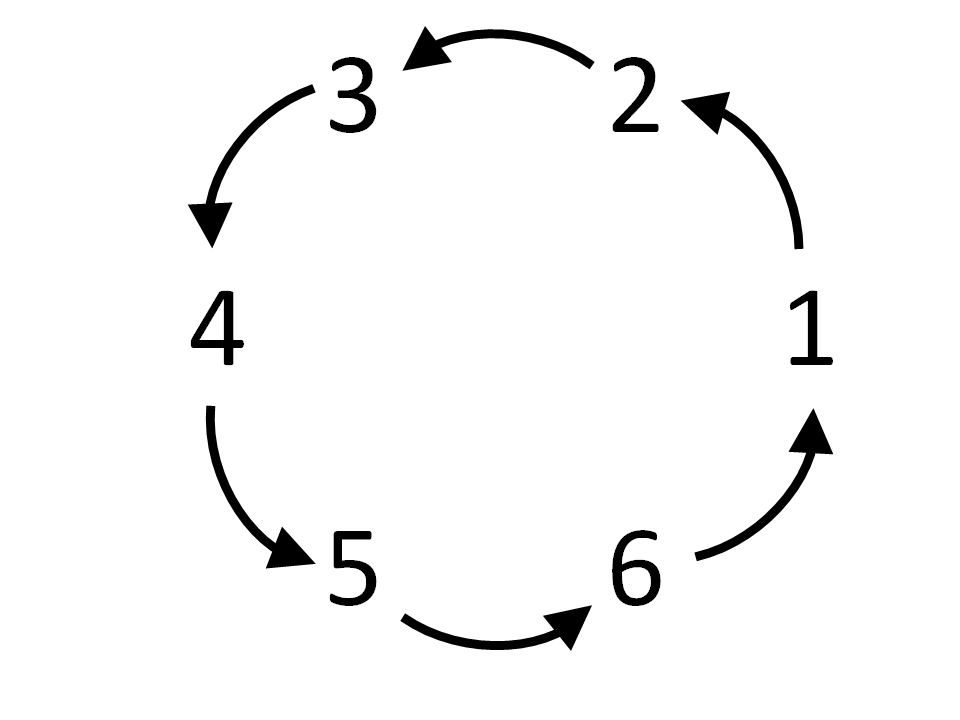
\includegraphics[width=1.25in]{images/perm_cycle.png}
\caption{Cycle representation of the  permutation (123456).}\label{fig:cycle}
\end{center}
\end{figure}

We shall write this trail of inputs and outputs as $(123456)$;\index{Cycle notation} and rather than ``wheel'', we call this a \bfii{ cycle}\index{Permutation!cycle}  Reading the cycle from left to right indicates that 1 goes to 2, 2 goes to 3, $\ldots$, and the 6 at the end goes back to 1.  %Note that according to this interpretation $(234561)$, or $(345612)$ are alternative ways of writing the same permutation..

\begin{exercise}\label{exercise:permute:equal_cycles2}
Show that $(123456) = (345612)$ by drawing a figure similar to Figure~\ref{fig:cycle}  for each cycle.
\end{exercise}

\begin{exercise}\label{exercise:permute:equal_cycles1}
Show that $(123456)$  and $(234561)$ both have the same tableau (so they are in fact the same permutation).
\end{exercise}

From the previous two exercises, it is clear that there are many ways to write the same cycle: we can begin with any element we ant, and work our way around until we get back to the same element. To avoid possible confusion, from now on we will follow the convention of starting the cycle with the ``smallest"  or ``first" element of the domain.

For this particular permutation, since our cycle contains all the inputs in the domain of $\rho$ it represents the whole function, because it gives us the outputs for every input.  Therefore in cycle notation, 
\[
\rho = (123456) \]
\end{example}

\begin{exercise}\label{exercise:permute:long_cycle_perm1}
Write the following permutation of $S_6$ in cycle notation:  
\[ \mu = \begin{pmatrix} 1 & 2 & 3 & 4 & 5 & 6 \\ 3 & 4 & 5 & 1 & 6 & 2 \end{pmatrix}. \]
\end{exercise}

\begin{exercise}\label{exercise:permute:long_cycle_perm2}
Given the permutation in $S_6$ $\mu = (152634)$:
\begin{enumerate}[(a)]
\item
Write $\mu$ in tableau form.
\item
Write $\mu$ as a figure similar to Figure~\ref{fig:cycle}
\end{enumerate}
\end{exercise}

\begin{exercise}\label{exercise:permute:long_cycle_perm3}
Given the permutation in $S_6$ $\mu = (165432)$:
\begin{enumerate}[(a)]
\item
Write $\mu$ in tableau form.
\item
Write $\mu$ as a figure similar to Figure~\ref{fig:cycle}
\item
Compare your answer to (b) with Figure~\ref{fig:cycle} of $\rho = (123456)$.  Explain the difference between $\mu$ and $\rho$. 
\end{enumerate}
\end{exercise}

\begin{defn} \label{cycle_length}
The \bfii{ length} of a cycle is how many elements the cycle contains; i.e. how many elements are in the parentheses\index{Cycle!length of}.  Formally, 
\begin{center}
if $(a_1, a_2, \ldots, a_n)$ is a cycle, then the length of $(a_1, a_2, \ldots, a_n) = n$.
\end{center}
\end{defn}
For example, the permutation $\rho$ in Example~\ref{example:permute:permute_to_cycle_1} above is represented by a cycle of length six.

\begin{rem}
Notice how we have used the notation $a_j$ to indicate arbitrary elements in a cycle.  This is a common practice in abstract algebra.
\end{rem}

Now not all permutations in $S_6$ correspond to a cycle of length six.  For instance:

\begin{example}\label{example:permute:permute_to_cycle_3}
Suppose $\tau \in S_6$ and $\tau  = \begin{pmatrix} 1 & 2 & 3 & 4 & 5 & 6 \\ 1 & 4 & 2 & 3 & 5 & 6 \end{pmatrix}$.  Then
\begin{itemize}
\item
$1 \to 1$, which means that $1$ ``stays put."  So we don't use $1$.
\item
$2 \to 4$, $4 \to 3$, and $3 \to 2$; so we have $(243)$.
\item
Finally, $5 \to 5$ and $6 \to 6$; so they also stay put.
\end{itemize}
Hence 
\[
\tau = (243) \]
\end{example}

Based on the procedure in the previous example then, how would we represent the identity permutation on a set of $n$ elements?  All the elements stay put, so technically ${\var id}$ would equal the ``empty cycle''.  Some references in fact use  ``$()$" to denote the identity: but in this book we will always denote
the identity permutation  by ${\var id}$ as a reminder that this is in fact the group's identity element.\index{Permutation!identity}\index{Identity!of permutation groups}

\begin{warn}
Cycle notation does not indicate the domain of the permutation. For instance, the permutation $(243)$ in Example~\ref{example:permute:permute_to_cycle_3} had domain $\{1,2,3,4,5,6\}$, but  $(243)$ could also refer to a permutation on the domain $\{1,2,3,4\}$. When working with permutations in cycle notation, make sure you know what the domain is. (In most cases, it's clearly specified by the context.)
% We must be very careful when working with and interpreting permutations in cycle notation.  $\tau$ only has three elements in its cycle, yet we know it has six elements in its domain.  What happened to the other elements?  Those single element parentheses were dropped because those elements "stayed put".  Therefore when we are given $\tau = (243)$, we must assume the other elements stay put.  Basically we assume the single parentheses are there, just like in the equation ''$3 + x = 8$'' we assume there is a 1 in front of $x$ though the coefficient isn't written.  However, what if I gave you $\tau$ without giving you the domain?  What elements, if any, can you assume stay put?  To make that assumption about $\tau$ we \emph{must} know the domain of $\tau$.  That \emph{cannot} be assumed, it must be known.
\end{warn}

\begin{exercise}\label{exercise:permute:short_cycle1}
Write each of the following permutations in $S_7$ in tableau form.
\begin{enumerate}[(a)]
\item
$\omega = (243)$
\item
$\omega = (2365)$
\item
$\omega = (14257)$
\end{enumerate}
\end{exercise}

\begin{exercise}\label{exercise:permute:short_cycle2}
Draw a figure similar to Figure~\ref{fig:cycle} depicting each of the following permutations in $S_5$.
\begin{enumerate}[(a)]
\item
$\sigma = (25)$
\item
$\sigma = (135)$
\item
$\sigma = (1342)$
\end{enumerate}
\end{exercise}
\noindent
A final question that may come to mind is,  Do all permutation correspond to some cycle?  Certainly, as we've seen, all cycles correspond to some permutation in $S_n$.  However, can all permutations in $S_n$ be represented as a cycle?  We will take the next several parts of this section to explore this question. 

\subsection{Composition (a.k.a. product) of cycles}

Since cycles represent permutations, they can be composed together.  If we change the cycles to tableaus, we know how to compose them.  Now let's figure out how to compose them using the cycles themselves.\index{Composition!of cycles}\index{Cycle!composition}

\begin{notation}{}
Given permutations $\sigma$ and $\tau$, instead of writing $\sigma \compose \tau$ we write the shorthand notation: $\sigma \tau$. Furthermore, instead of calling this the composition of $\sigma$ and $\tau$, we refer to it as the \bfii{ product} of $\sigma$ and $\tau$.
\footnote{Once again we see mathematicians'  annoying habit of  reusing familiar terms to mean something new  in a different contexts. In this case,  the ``product'' of permutations has nothing at all to do with multiplication.}
\end{notation}

\begin{example}\label{example:permute:cycle_comp_1}
Suppose we want to form the product (that is, composition)
 $\sigma \tau$, where $\sigma, \tau \in S_6$ and
$\sigma  = (1 5 3 2 ),
\tau    = (1 2 6)$.

\begin{figure}[ht]
\begin{center}
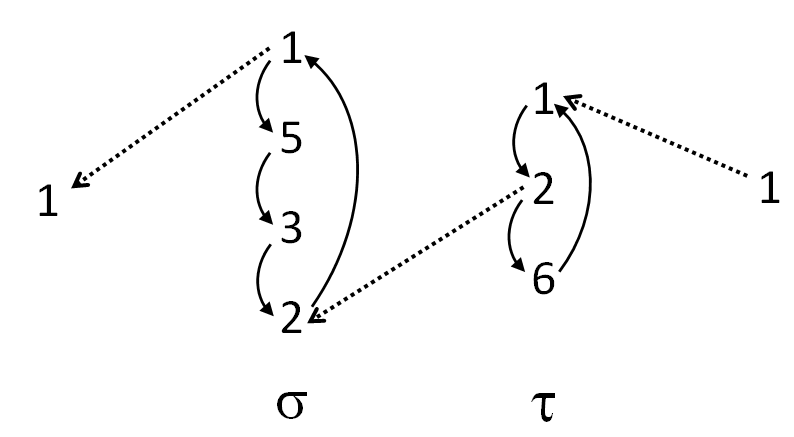
\includegraphics[width=2.0in]{images/cycle_composition.png}
\caption{Product of cycles $\sigma$ and $\tau$, showing the derivation of $\sigma \tau (1) = 1$.}
\label{fig:cycle_composition}
\end{center}
\end{figure}

Figure~\ref{fig:cycle_composition} provides a visual representation of how the product $\sigma \tau$ acts on 1. Remember that we operate from right to left, so the figure shows `1' coming in from the right. The action of  $\tau$ takes 1 to 2. ( For convenience we have ``flattened'' the permutations $\tau$ and $\sigma$, so they no longer appear as circles.) Then we pass over to $\sigma$, which takes 2 to 1.  The final result is 1: therefore $\sigma(\tau(1)) = 1$.

Evidently 1 remains unchanged by the permutation, so let's look at what happens to 2. We see this in  Figure~\ref{fig:cycle_composition2}.  First, $\tau$ moves 2 to 6. Moving on to $\sigma$, we find that $\sigma$ leaves the 6 unchanged. The result is that $\sigma(\tau(2)) = 6$.

\begin{figure}[ht]
\begin{center}
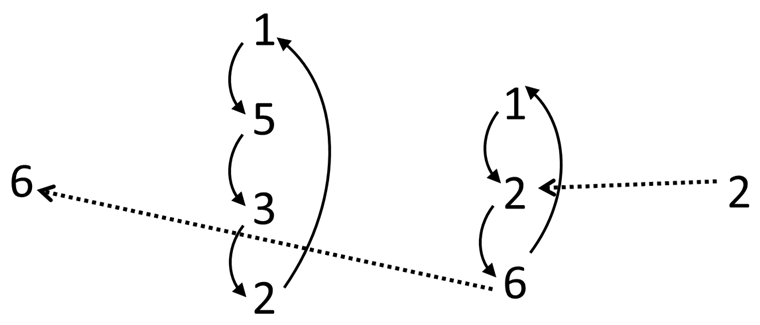
\includegraphics[width=2.0in]{images/cycle_composition_2.png}
\caption{Product of cycles $\sigma$ and $\tau$ (continued), showing $\sigma \tau (2) = 6$.}
\label{fig:cycle_composition2}
\end{center}
\end{figure}
We have seen that $\sigma\tau$ takes 2 to 6: so now let's see where $\sigma\tau$ takes 6. (Perhaps you can see that we're trying to build a cycle here.)  
The top part of Figure~\ref{fig:cycle_composition_finish} uses the same process to show the result:  $\sigma(\tau(6)) = 5$.  
The middle part of Figure~\ref{fig:cycle_composition_finish} shows that $\sigma(\tau(5)) = 3$; and the bottom part of Figure~\ref{fig:cycle_composition_finish} shows that $\sigma(\tau(3)) = 2$. We already know that $\sigma(\tau(2)) = 6$, so we have closed out our cycle. We have shown $2 \rightarrow 6  \rightarrow 5  \rightarrow 3  \rightarrow 2$, which amounts to the cycle: $(2653)$.

\begin{figure}[ht]
\begin{center}
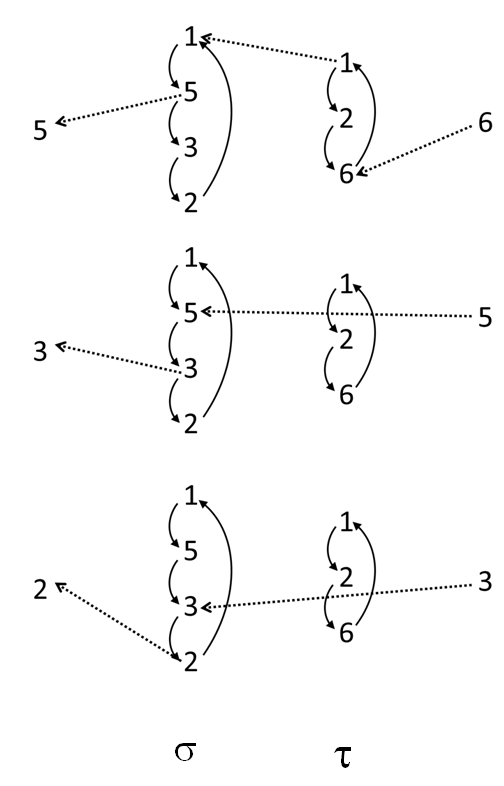
\includegraphics[width=2.0in]{images/cycle_composition_finish.png}
\caption{Product of cycles $\sigma$ and $\tau$ (continued), showing $6\rightarrow5\rightarrow3\rightarrow2$.}
\label{fig:cycle_composition_finish}
\end{center}
\end{figure}
So far 4 is unaccounted for: but a quick inspection of Figure~\ref{fig:cycle_composition_finish} shows that 4 is not affected by either $\tau$ or $\sigma$.  
So  the entire action of $\tau$ followed by $\sigma$  is summarized by the cycle $(2653)$, meaning that we can write: $\sigma \tau$  = $(2653)$.
\end{example}

\begin{exercise}\label{exercise:permute:perm_not_comm}
Using the same permutations $\sigma$ and $\tau$ as above:
\begin{enumerate}[(a)]
\item
Write the product $\tau \sigma$ in cycle notation.
\item
By comparing your results for $\sigma \tau$ and $\tau \sigma$, fill in the blank in the following statement:  In general, permutations do not $\_\_\_\_\_\_\_\_\_\_\_\_$.
\end{enumerate}
\end{exercise}

\begin{example}\label{example:permute:cycle_comp_2a}
At the beginning it may be helpful to draw a picture, as in the previous example. However, once you gain experience, you should be able to find the product of cycles directly.  Consider the product  $\sigma\tau$ where $\sigma = (AEDBF)$ and $\tau=(ABDFE)$.  Then we have:

\begin{itemize}
\item
$\tau$ takes $A \to B$  and $\sigma$ takes $B \to $F; hence $\sigma \tau$ takes $A \to F$.
\item
$\tau$ takes $F \to E$, and $\sigma$ takes $E \to D$; hence $\sigma \tau$ takes $F \to D$.
\item
$\tau$ takes $D \to F$, and $\sigma$ takes $F \to A$; hence $\sigma \tau$ takes $D \to A$.
\end{itemize}
We have finished a cycle:  $(AFD)$.  Let us check where the other letters $B, C, E$ go:
\begin{itemize}
\item
$\tau$ takes $B \to D$, and $\sigma$ takes $D \to B$; hence $\sigma \tau$ takes $B \to B$.
\item
Neither $\tau$ nor $\sigma$ affects $C$; hence $\sigma \tau$ takes $C \to C$.
\item
$\tau$ takes $E \to A$, and $\sigma$ takes $A \to E$; hence $\sigma \tau$ takes $E \to E$.
\end{itemize}
Since $B, C, E$ are unaffected by $\sigma \tau$, we conclude that $\sigma \tau=(AFD)$.
\end{example}

\begin{exercise}\label{exercise:permute:cycle_comp_exer1}
Given that $\delta = (135)$, $\sigma = (347)$, and $\rho = (567)$ are permutations in $S_7$, compute the following:
\begin{multicols}{3}
\begin{enumerate}[(a)]
\item
$\delta \sigma$
\item
$\sigma \delta$
\item
$\delta \rho$
\item
$\rho \delta$
\item
$\sigma \rho$
\item
$\rho \sigma$
\end{enumerate}
\end{multicols}
\end{exercise}

\subsection{Product of disjoint cycles}

%Though in general the product of cycles is not commutative, their are particular types of cycles that are commutative under function composition.

\begin{defn} \label{disjoint_cycles} 
Two cycles are \bfii{ disjoint} if their parentheses contain no elements in common.  Formally,
two cycles $(a_1, a_2, \ldots, a_k )$ and $(b_1, b_2, \ldots, b_l )$, are \bfii{ disjoint}\index{Cycle!disjoint}
if $a_i \neq b_j, \forall i, j $ such that $1 \le i \le k$ and $1 \le j \le l$. 
\end{defn}

\noindent
For example, the  cycles $(135)$ and $(27 )$ are disjoint, whereas the cycles
$(135)$ and $(347 )$ are not.  

\begin{example}\label{example:permute:cycles_disjoint_comp}
Given $\sigma = (135)$, $\tau = (27)$, and $\sigma , \tau \in S_7$. Let us compute $\sigma \tau$. 
We may  do this using the following diagram:
\[ \text{home}~\leftarrow~\underbrace{\sigma}_{(1 3 5)} \leftarrow \underbrace{\tau}_{(27)} ~\leftarrow~\text{home} \]
Take each number in $\{1,2,3,4,5,6,7\}$, start from ``home'' on the right, and pass through the two ``coatrooms''  
$\tau$ and $\sigma$ one by one.  If the number agrees with one of the numbers in the first ``coatroom'', then the number ``changes its coat'' and turns into the next number in the list.  Then, it passes to the next ``coatroom'' where it does the same thing. Once it reaches ``home'' on the left, we have the result of $\sigma \tau$ acting on the original number.
%
%
%\begin{figure}[ht]
%\begin{center}
%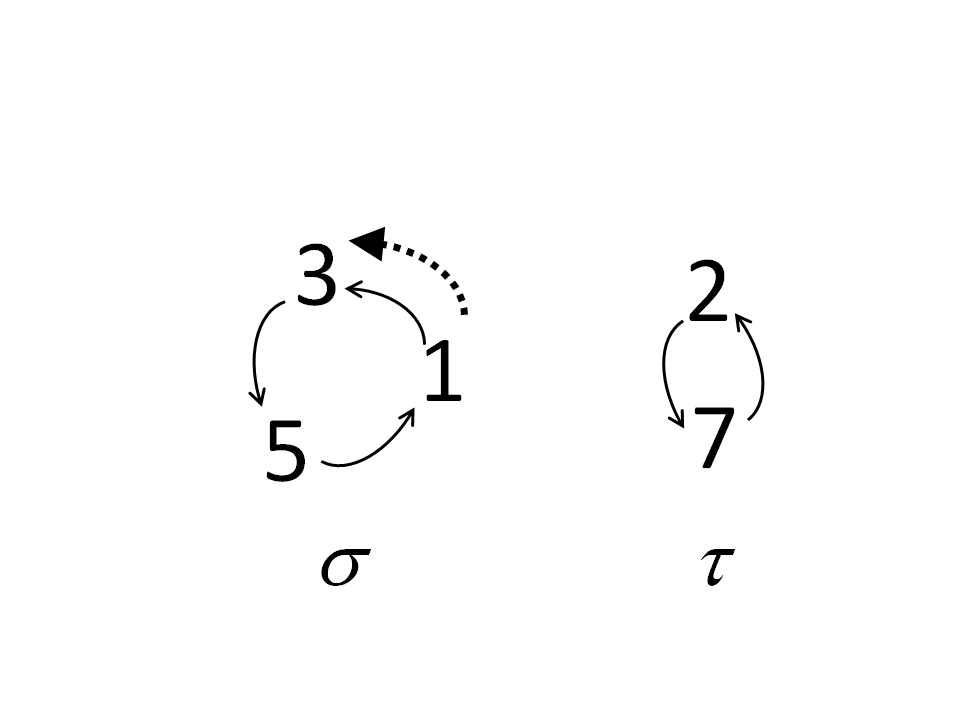
\includegraphics[scale=0.2]{images/disjoint_cycle_composition.png}
%\caption{Product of disjoint cycles $\sigma$ and $\tau$, showing the derivation of $\sigma \tau (1)=3$}\label{fig:disjoint_cycle_composition}
%\end{center}
%\end{figure}
%
%\begin{itemize}
%\item
%$\tau$ takes $1 \to 1$, then $\sigma$ takes $1 \to 3$; therefore $1 \to 3$.
%\item
%$\tau$ takes $3 \to 3$, then $\sigma$ takes $3 \to 5$; therefore $3 \to 5$.
%\item
%$\tau$ takes $5 \to 5$, then $\sigma$ takes $5 \to 1$; therefore $5 \to 1$. 
%\end{itemize}
%
%\noindent
%So far, we have the cycle  $(135)$.  Let's continue with the other inputs:
%\begin{itemize}
%\item
%$\tau$ takes $2 \to 7$, then $\sigma$ takes $7 \to 7$; therefore $2 \to 7$.
%\item
%$\tau$ takes $7 \to 2$, then $\sigma$ takes $2 \to 2$; therefore $7 \to 2$.
%\end{itemize}
%
%\noindent
%So we have another cycle, $(27)$.  Finally, %both $\tau$ and $\sigma$ keep 4 and 6 put; therefore $4 \to 4$ and $6 \to 6$.

Notice that every number affected by $\tau$ is unaffected by $\sigma$; and vice versa. Since the two cycles always  remain separate, it is appropriate to represent $\sigma \tau$ as $(135)(27)$, because the cycles don't reduce any farther.
\end{example}

This example also illustrates another point.  Since $S_7$ is closed under function composition, it follows that $\sigma \tau$ must be a permutation in $S_7$.

\begin{exercise}
Write the permutation $\sigma \tau$ from Example~\ref{example:permute:cycles_disjoint_comp} in tableau form.
\end{exercise}

This permutation can't be represented by one cycle, but rather by \emph{two} disjoint cycles.  So we have an answer to our previous question: all cycles are permutations, but not all permutations are cycles.  Some are represented by two disjoint cycles: and in fact some are represented by more than two disjoint cycles.

\begin{example}\label{example:permute:permute_to_cycle_2}
Suppose $\mu \in S_7$ and $\mu = \begin{pmatrix} 1 & 2 & 3 & 4 & 5 & 6 & 7 \\ 6 & 1 & 4 & 3 & 7 & 2 & 5 \end{pmatrix}$.  Then
\begin{itemize}
\item
$1 \to 6$, $6 \to 2$, and $2 \to 1$;  therefore we have the cycle $(162)$.
\item
$3 \to 4$ and $4 \to 3$; therefore we have $(34)$. 
\item
Finally, $5 \to 7$ and $7 \to 5$; therefore we have $(57)$. 
\end{itemize}

\noindent
Hence $\mu = (162)(34)(57)$, as we may verify by computing the product $(162)\compose (34)\compose (57)$ directly.

We may represent this process graphically as follows. The permutation $\mu$ is also a binary relation, and thus can be represented as a digraph as shown in Figure~\ref{permute:cycle_rep}(a). We can make the digraph appear much simpler by rearranging the vertices as in Figure~\ref{permute:cycle_rep}(b). We shall see that \emph{all} permutations can be simplified in this manner.\index{Digraph!of a permutation}
\end{example}

\begin{figure}[ht]
\begin{center}
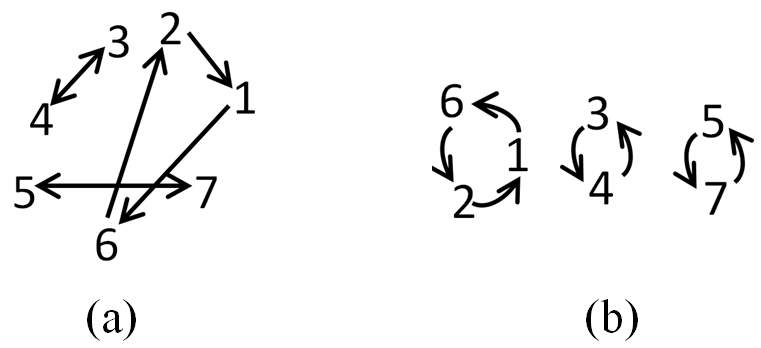
\includegraphics[width=2.25in]{images/cycle_rep.png}
\caption{(a) Digraph representation of permutation (b) Rearrangement of digraph into cycles}\label{permute:cycle_rep}
\end{center}
\end{figure}

%Here is a summary of the steps for converting a tableau to cycle notation.
%\begin{itemize}
%\item
%First we apply the permutation to the "beginning" element of our domain.  
%\item
%Next, we repeatedly applying the permutation to the resulting outputs, until we get back to the beginning element.  
%\item
%Then, if there are elements of the domain left out, we start with one of the elements left out and follow that element until we return to it.  
%\item
%We continue doing the last step until we've accounted for all the elements in the permutation's domain.
%\end{itemize} 

\begin{exercise}\label{exercise:permute:tab_to_cycle}
Write the following permutations in cycle notation.
\begin{multicols}{2}
\begin{enumerate}[(a)]
 
\item
\[ \rho =
\begin{pmatrix}
1 & 2 & 3 & 4 & 5 & 6  \\
2 & 1 & 5 & 6 & 3 & 4 
\end{pmatrix}
\]

\item
\[ \sigma =
\begin{pmatrix}
1 & 2 & 3 & 4 & 5 & 6\\
2 & 5 & 6 & 4 & 1 & 3
\end{pmatrix}
\]

\item
\[ \omega =
\begin{pmatrix}
1 & 2 & 3 & 4 & 5 & 6 \\
4 & 5 & 1 & 6 & 2 & 3
\end{pmatrix}
\]

\item
\[ \tau =
\begin{pmatrix}
1 & 2 & 3 & 4 & 5 & 6 \\
5 & 3 & 4 & 1 & 2 & 6
\end{pmatrix}
\]

\end{enumerate}
\end{multicols}
\end{exercise}

\begin{exercise}\label{exercise:permute:cycle_to_tab}
Write each of the following permutations in $S_9$ in tableau form.
\begin{multicols}{2}
\begin{enumerate}[(a)]
\item
$\mu = (259)(347)$.
\item
$\sigma = (25678)(14)(39)$.
\item
$\tau = (286)(193)(457)$.
\item
$\omega = (257)(18)$.
\end{enumerate}
\end{multicols}
\end{exercise}

\begin{exercise}\label{exercise:permute:D6_cycles}
Write the permutations of $D_6$ in cycle notation (recall that $D_6$ is the group of symmetries of a hexagon).
\end{exercise}

\begin{exercise}\label{exercise:permute:D4_cycles}
Write the symmetries of a square in cycle notation.
\end{exercise}

There is one more issue we need to explore with the product of disjoint cycles, which we will do in the following exercise.

\begin{exercise}\label{exercise:permute:dis_cycles_comm}
In parts (a)--(d) below, write both permutations on the set \{1,2,3,4,5,6\} in tableau form.
\begin{enumerate}[(a)]
\begin{multicols}{2}
 \item
$(123)(45)$ and $(45)(123)$.
\item
$(14)(263)$ and $(263)(14)$
\item
$(1352)(46)$ and $(46)(1352)$
\item
$(135)(246)$ and $(246)(135)$
\end{multicols}
\item
From your results in (a)-(d), what do you conjecture about the product of disjoint cycles?
\end{enumerate}
\end{exercise}
The examples in Exercise~\ref{exercise:permute:dis_cycles_comm} seem to indicate that the product of disjoint cycles is commutative. This is in fact true, as we shall now prove.\index{Commutative property!of disjoint cycles}
 
\begin{prop}\label{proposition:permute:disjoint_cycles_commute}
Disjoint cycles commute: that is, given two disjoint cycles $\sigma = (a_1, a_2, \ldots, a_j)$ and $\tau = (b_1, b_2, \ldots, b_k)$ we have
\[
\sigma \tau = \tau \sigma = (a_1, a_2, \ldots, a_j) (b_1, b_2, \ldots, b_k) \]
\end{prop}

\begin{proof} We present this proof as a fill-in-the-blanks exercise:

\begin{exercise}\label{exercise:permute:disjoint_commutative} Fill in the $\underline{<\#>}$  to complete the proof:

Recall that permutations are defined as bijections on a set $X$. In order to show that the two permutations 
$\sigma \tau$ and $\tau \sigma$ are equal, it's enough to show that they are the same function. In other words, we just need to show that $\sigma \tau (x)$ =\underline{ $~<1>~$} for all $x \in X$.

We'll define $A = \{a_1, a_2, \ldots, a_j\}$ and $B = \{b_1, b_2, \ldots, b_k\}$. By hypothesis $A$ and $B$ are disjoint, so $A \underline{ ~<2>~} B = \underline{ ~<3>~}$. Given an arbitrary $x \in X$, there are three possibilities: (i) $x \in A$ and $x \notin B$; (ii) $x \in \underline{ ~<4>~}$ and $x \notin \underline{ ~<6>~}$; (iii) $x \notin \underline{ ~<7>~}$ and $x \notin \underline{ ~<8>~}$. 

\begin{enumerate}[(i)]
\item
In this case, since $x \notin B$ it follows that $\tau(x) = x$. We then have $\sigma \tau (x) = \sigma(\tau(x)) = \sigma(x)$. Furthermore, since $x \in A$ it follows that $\sigma(x) \in A$, so $\sigma(x) \notin B$. We then have $\tau \sigma (x) = \tau(\sigma(x)) = \sigma(x)$. It follows that $\sigma \tau (x) = \tau \sigma (x)$.
\item
In this case, since $x \notin \underline{ ~<9>~}$ it follows that $\underline{ ~<10>~}(x) = x$. We then have $\tau \sigma (x) = \underline{ ~<11>~} = \underline{ ~<12>~}(x)$. Furthermore, since $x \in \underline{ ~<13>~}$ it follows that $\underline{ ~<14>~}(x) \in \underline{ ~<15>~}$, so $\underline{ ~<16>~}(x) \notin \underline{ ~<17>~}$. We then have $\sigma \tau (x) = \underline{ ~<18>~} = \underline{ ~<19>~}(x)$. It follows that $\sigma \tau (x) = \tau \sigma (x)$.
\item
In this case, since $x \notin A$ it follows that $\underline{ ~<20>~}(x) = x$. Similarly since $x \notin \underline{ ~<21>~}$ it follows that $\underline{ ~<22>~}(x) = x$.We then have $\tau \sigma (x) = \underline{ ~<23>~}$ and $\sigma \tau (x) = \underline{ ~<24>~}$. It follows that $\sigma \tau (x) = \tau \sigma (x)$.
\end{enumerate}

\noindent
In all three cases we have $\sigma \tau (x)$ = $\underline{ ~<25>~}$, so therefore $\sigma \tau = \tau \sigma$.
\end{exercise}
\end{proof}

\noindent
What we've discovered about products of two disjoint cycles is also true for products of any number of disjoint cycles. Since disjoint cycles act independently, they all commute.

\begin{exercise}
Write each of the following permutations on $X = \{1,2,\ldots,9\}$ in tableau form.
\begin{enumerate}[(a)]
\begin{multicols}{3}
\item
$(1346)(298)(57)$
\item
$(57)(1346)(298)$
\item
$(298)(57)(1346)$
\end{multicols}
\item
Which of the above permutations are the same? Which are different? \emph{Explain} your answer.
\end{enumerate}
\end{exercise}

\begin{exercise}
Write each of the following permutations 3 different ways using cycle notation.
\begin{enumerate}[(a)]
\begin{multicols}{3}
\item
$(147)(258)(369)$
\item
$(12)(35)(46)(78)$
\item
$(14359)(28)(67)$
\end{multicols}
\end{enumerate}
\end{exercise}


\subsection{Products of permutations using cycle notation}
Finally, now that we know how to deal with permutation compositions that simplify to disjoint cycles, we can now compose any set of permutations we want.  Let us begin with a relatively small example.

\begin{example}\label{example:permute:cycle_comp_3}
Given the permutations $\mu = (257)(134)$ and $\rho = (265)(137)$ in $S_7$, write $\mu \rho$ in cycle notation.

This is actually not that much different from what we've done already. Using our ``coatroom'' representation, we have:

\[ \text{home}~\leftarrow~\underbrace{(257)\leftarrow (134)}_{\mu} \leftarrow \underbrace{(265)\leftarrow (137)}_{\rho} ~\leftarrow~\text{home} \]
We have written arrows between the cycles in $\mu$ and $\rho$ to emphasize that in this case we essentially have four coatrooms, one after the other. So starting from the right with 1, we have
%
%
%In Figure~\ref{fig:cycle_comp3}, we have represented $\mu \rho$ by placing the cycle representations side-by-side.   . Starting from the right:
%
%
%\begin{figure}[ht]
%\begin{center}
%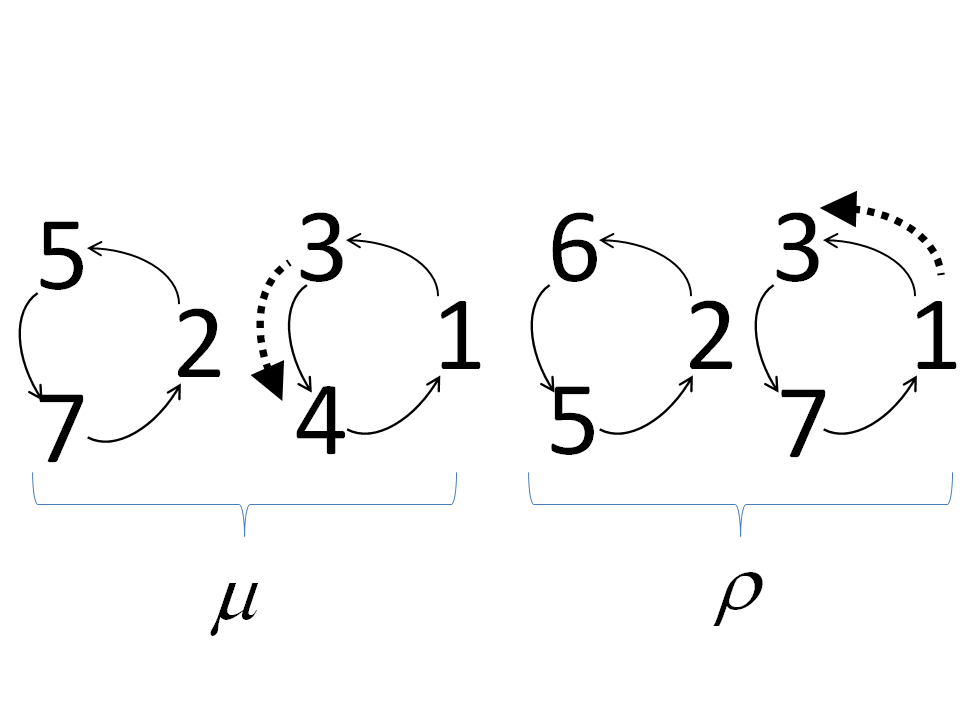
\includegraphics[scale=0.2]{images/cycle_comp3.png}
%\caption{Product of permutations $\mu$ and $\rho$, showing the derivation of $\mu \rho(1) = 4$}\label{fig:cycle_comp3}
%\end{center}
%\end{figure}
%

\begin{itemize}
\item
$1 \to 3$, $3 \to 3$, $3 \to 4$, and $4 \to 4$; therefore $1 \to 4$.
\item
$4 \to 4$, $4 \to 4$, $4 \to 1$, and $1 \to 1$; therefore $4 \to 1$. 
\end{itemize}

\noindent
This gives us the cycle $(14)$.  Continuing,
\begin{itemize}
\item
$2 \to 2$, $2 \to 6$, $6 \to 6$, and $6 \to 6$; therefore $2 \to 6$.
\item
$6 \to 6$, $6 \to 5$, $5 \to 5$, and $5 \to 7$; therefore $6 \to 7$.
\item
$7 \to 1$, $1 \to 1$, $1 \to 3$, and $3 \to 3$; therefore $7 \to 3$.
\item
$3 \to 7$, $7 \to 7$, $7 \to 7$, and $7 \to 2$; therefore $3 \to 2$.
\end{itemize}

\noindent
So we have the cycle  $(2673)$.  Now the only input not included in our cycles is $5$, so logically it should stay put.  But let's test it just in case we made a mistake in our work above.
\begin{itemize}
\item
$5 \to 5$, $5 \to 2$, $2 \to 2$, and $2 \to 5$; therefore $5$ does indeed stay put.
\end{itemize}

\noindent
So, we finally have:  $\mu \rho = (14)(2673)$
\end{example}

\begin{example}\label{example:permute:cycle_comp_4}
Find the product $(156)(2365)(123)$  in $S_6$ .
\begin{itemize}
\item
$1 \to 2$, $2 \to 3$, and $3 \to 3$; therefore $1 \to 3$.
\item
$3 \to 1$, $1 \to 1$, and $1 \to 5$; therefore $3 \to 5$.
\item
$5 \to 5$, $5 \to 2$, and $2 \to 2$; therefore $5 \to 2$.
\item
$2 \to 3$, $3 \to 6$, and $6 \to 1$; therefore $2 \to 1$.
\end{itemize}

\noindent
So we have $(1352)$.

\begin{itemize}
\item
$4$ does not appear in any of the cycles, so we know it won't be acted on by any of the cycles.  Hence $4$ stays put.
\item
$6 \to 6$, $6 \to 5$, and $5 \to 6$; hence $6$ stays put.
\end{itemize}

\noindent
Therefore $(156)(2365)(123) = (1352)$.
\end{example}

\begin{exercise}\label{exercise:permute:cycle_comp_5}
Given the following permutations in $S_8$, 

\[  \sigma = (1257)(34) , \tau = (265)(137), \text { and } \rho = (135)(246)(78) \]

\noindent
write the following in cycle notation:
\begin{enumerate}[(a)]
\begin{multicols}{2}
\item
$\sigma \tau$
\item
$\tau \sigma$
\item
$\tau \rho$
\item
$\sigma \rho$
\end{multicols}
\end{enumerate}
\end{exercise}



\begin{exercise}\label{exercise:permute:cycle_comp_2}
Compute each of the following.
\begin{multicols}{3}
\begin{enumerate}[(a)]
 \item
$(1345)(234)$
\item
$(12)(1253)$
\item
$(143)(23)(24)$
\item
$(1423)(34)(56)(1324)$
\item
$(1254)(13)(25)$
\item
$(1254) (13)(25)^2$
\item
$(1254)^2 (123)(45)$
\end{enumerate}
\end{multicols}
\end{exercise}


%\noindent
%In fact, if we apply the cycle product computation procedure to \emph{any} product of cycles, the result will be a set of \emph{disjoint} cycles. 
%
%So the following proposition should be no surprise.
%%%%This disjoint cycle business really should be moved to right after cycle composition

%\begin{prop}\label{proposition:permute:disjoint_cycle_representation}
%Any permutation can be represented as a product of disjoint cycles.
%\end{prop}
%\begin{proof} \emph{(Informal)} 
%Any permutation $\mu$ acting on a set $X$ can be written in tableau form. Then I claim that the procedure in Examples~\ref{example:permute:permute_to_cycle_1}~--~\ref{example:permute:permute_to_cycle_1}  applied to the tableau form of $\mu$ is guaranteed to produce a equivalent representation as a product of disjoint cycles. "Why are the cycles disjoint?" you may ask.  Good question! Well, suppose the procedure applied to $\mu$ yields the following cycles:
%
%\[ \mu = (a_1 a_2 \cdots a_i)(b_1 b_2 \cdots b_j) (c_1 c_2 \cdots c_k) \ldots . \]
%
%\noindent
%Suppose for instance that the first and third cycle have elements in common: that is, suppose $c_n = a_m$. Then  since $\mu$ is a bijection we have $\mu^{-1}(c_n) = \mu^{-1}(a_m)$, so by construction $c_{n-1} = a_{m-1}$. This fact can be applied repeatedly to obtain that $c_1 = a_p$ for some $p$ where $1 \le p \le i$. But the procedure specifies that $c_1$ cannot be in any previous cycle. This is a contradiction: therefore the first and third cycles have no elements in common. The same argument goes to show that any two cycles in the representation will be disjoint.
%\end{proof}




%The product of two cycles that are not disjoint may reduce to something less complicated; but, in our experience so far, the product of disjoint cycles never reduces to a simplified form.  This makes intuitive sense, because since disjoint cycles don't have any elements in common, each cycle doesn't'affect the elements in the other cycle during composition.  For example, if I start my first composition above with say element 5, the cycle $(2 7)$ keeps that element the same, while $(1 3 5)$ moves $5 \to 1$.  The same thing happens with 1 and 3, and hence the cycle $(1 3 5)$ is left unchanged.  Similarly, the composition leaves $(2 7)$ unchanged.  

%Also, we can see that if we reversed the order of composition for the disjoint cycles, $(2 7)(1 3 5) = (1 3 5)(2 7)$.  Since the cycles do not affect each other, then switching the order we compose them in leaves the total effect of the composition unchanged (2 still goes to 7, 1 goes to 3, etc.).  Hence while cycle composition is not usually commutative ($(1 3 5)(3 4 7) \neq (3 4 7)(1 3 5)$), the composition of \emph{disjoint} cycles is commutative.  
%
% CPT it would be good to provide a proof.
%We state these facts about disjoint cycles in the following proposition, without general proof. 

\subsection{Cycle structure of permutations}

Over the last several subsections, we've seen permutations represented as no cycles (${\var id}$), one cycle, or the product of any number of disjoint cycles.  This worked because both a single cycle and a product of disjoint cycles can't be reduced to a simpler form in cycle notation.  Are there any other possibilities?   Are there permutations that can't be represented as either a single cycle or a product of disjoint cycles?  The answer to this compelling question is given in the following proposition. 

%%% I don't think it's necessary to include the following
% For instance, suppose there was a permutation that couldn't be represented by either a one-cycle or $n$ disjoint cycles.  Then it would have to be represented by more than one cycle, say $k$ cycles, in which $m$ (at least two) of the cycles are disjoint.  But if this was the case, then by our work so far, we know we could take the $m$ disjoint cycles and simplify them, two at a time, to either one-cycle or say $p$ disjoint cycles.  Either way, our permutation would then be represented by either a one-cycle or $(k - m + p)$ disjoint cycles.  This then is an informal, not fully generalized explanation (short of a proof) for the following fact:

\begin{prop}\label{proposition:permute:perm_simple_notation}     
Every permutation in $S_n$ can be written either as the identity, a  single cycle, or as the product of disjoint cycles. 
\end{prop}

\noindent
The following  proof is a formalized version of the procedure we've been using to change permutations from tableau form to cycle notation.
Admittedly, it looks intimidating. However, we include it for your ``cultural enrichment'', because higher-level  mathematics is typically  like this. It's often the case that  particular examples of a certain principle are relatively easy to explain, but constructing a  general proof that covers \emph{all} cases is much more difficult.

\medskip
\noindent
Also, recall  that the notation $\sigma = (a_1, a_2, \ldots, a_n)$ means:
\begin{align*}
\sigma( a_1 )  = a_2  & &
\sigma( a_2 )  = a_3 & 
 \ldots   & \ldots & 
\sigma( a_k )  = a_1,
\end{align*}

\noindent
and $\sigma( x) =x$ for all other elements $x \in X$.


\begin{proof}
We can assume that $X = \{ 1, 2, \ldots, n \}$. Let $\sigma \in S_n$,
and define $X_1 = \{1,  \sigma(1), \sigma^2(1), \ldots \}$. The set $X_1$ is finite since $X$ is finite. Therefore the sequence  $1, \sigma(1), \sigma^2(1), \ldots $ must repeat. Let $j_1$ be the first index where the sequence repeats: that is, $\sigma^{j_1}(1) = \sigma^k(1)$ for some $k < j_1$.  Then if we apply $\sigma^{-1}$  to both sides of the equation we get 
$\sigma^{j_1-1}(1) = \sigma^{k-1}(1)$. Repeating this $k-1$ more times gives $\sigma^{j_1-k}(1) = 1$. This implies that the sequence repeats at index $j_1-k$: but we've already specified that $j_1$ is the \emph{first} index where the sequence repeats. The only way this can happen is if $k=0$. It follows that $X_1 = \{1, \sigma(1), \sigma^2(1), \ldots \sigma^{j_1-1}(1) \}$, where $\sigma^j_1(1) = 1$.

Now there are two possible cases: 

\begin{enumerate}[(i)]
\item
$X_1$ accounts for all the integers in $X$; i.e. $X_1 = X$ 
\item
there are some integers in $X$ not accounted for in $X_1$ (that is, $X \backslash X_1 \neq \emptyset$).  
\end{enumerate}

If case (ii) holds, then  let $i$ be the smallest integer
in $X \backslash X_1$ and define $X_2$ by $\{ i, \sigma(i),
\sigma^2(i), \ldots \}$. Just as with $X_1$, we may conclude that $X_2$ is a finite set, and that $X_2$ = $\{ i, \sigma(i), \ldots, \sigma^{j_2-1}(i) \}$ where $\sigma^{j_2}(i) = i$.

We claim furthermore that  $X_1$ and $X_2$ are disjoint. We can see this by contradiction: \emph{suppose} on the other hand that $X_1$ and $X_2$ are not disjoint. Then it must be the case that $\sigma^p(1) = \sigma^q(i)$ for some natural numbers $p, q$ with $0 \le p < j_1$ and $0 \le q < j_2$. Applying $\sigma$ to both sides of this equation, gives $\sigma^{p+1}(1) = \sigma^{q+1}(i)$. If we  continue applying $\sigma$ to both sides a total of $j_2 - q$ times then we obtain $\sigma^{p+j_2 - q}(1) = \sigma^{j_2}(i)$. But since $\sigma^{j_2}(i) = i$, it follows that $\sigma^{p+j_2 - q}(1) = i$, which implies that $i \in X_1$. This is a contradiction, because we know $i \in X \backslash X_1$. The contradiction shows that the \emph{supposition} must be false, so $X_1$ and $X_2$ are disjoint.

Continuing in
the same manner, we can define finite disjoint sets $X_3, X_4, \ldots$.
Since $X$ is a finite set, we are guaranteed that this process will
end and there will be only a finite number of these sets, say $r$. If
$\sigma_i$ is the cycle defined by 
\[
\sigma_i( x )
= \left\{
\begin{array}{ll}
\sigma( x ) & x \in X_i \\
x & x \notin X_i,
\end{array}
\right.
\]
then $\sigma = \sigma_1 \sigma_2 \cdots \sigma_r$. Since the sets
$X_1, X_2, \ldots, X_r$ are disjoint, the cycles $\sigma_1, \sigma_2,
\ldots, \sigma_r$ must also be disjoint.  

Now recall case (i) above. In this case,  $\sigma = \sigma_1$.  Hence, $\sigma$ is either a single cycle or the product of $r$ disjoint cycles.

Note that this proof also works in case $\sigma = {\var id}$: In this case all of the $X_m$'s are single-element sets, and each cycle has length 1.
\end{proof}
\medskip

% CPTshow cycle structure is unique? (in the sense that every cycle in one rep must be a cycle in the other rep, and vice versa)
Proposition~\ref{proposition:permute:perm_simple_notation} is a \emph{classification theorem}. You have seen classification theorems before: for instance, you know that any natural number $>1$ can be written uniquely as the product of primes.  Proposition~\ref{proposition:permute:perm_simple_notation} similarly gives us a standard way to represent permutations. It allows us to characterize the types of permutations in $S_n$ according to their cycle sizes, as shown in the following example.

\begin{example}\label{example:permute:S5_cycle_types}
We know that every permutation in $S_5$ is the product of disjoint cycles. Let us list all  possible cycle lengths and number of cycles for the permutations of $S_5$.
\begin{itemize}
\item
First of all, $S_5$ contains the identity, which has no cycles.
\item
Second, some permutations in $S_5$ consist of a single cycle.  The single cycle could have length 2, 3, 4, or 5 (remember, we don't count cycles of length 1).
\item
Third, some permutations in $S_5$ consist of the product of two disjoint cycles. To enumerate these, suppose first that one of the cycles is a cycle of length 2. Then the other cycle could be a cycle of length 2 (for instance in the case $(12)(34)$) or a cycle of length 3 (as in the case $(14)(235)$). There are no other possibilities, because we only have 5 elements to permute, and a larger disjoint cycle would require more elements.
\item
It's not possible to have three or more disjoint cycles, because that would require at least six elements.
\end{itemize}

%%% CPT commented following out
% For instance, some of the permutations will be represented by a one-cycle.  Now what are the possible lengths of these one-cycle permutations?  We are permuting a set of five elements, so we will have one-cycles of length 5.  Now there are also one-cycle permutations that keep one element from changing; hence we will have one-cycles of length 4.  Similarly, we will have one-cycles of length 3 and 2.  Why not a one-cycle of length 1 you say?  A one-cycle of length 1 keeps all the elements unchanged; therefore a one-cycle of length 1 is just the identity.  There are other ways though to describe the identity, for instance as a 5-cycle, each cycle of length 1; therefore in determining the types of permutations, we just list the identity by itself.

% Now that we've dealt with all the types of one-cycles, lets delineate all the types of two cycles.  Since we're permuting on 5 elements, the lengths of our cycles must add up to 5.  Therefore we could have a two-cycle of length 2 and 3.  We could also keep one element fixed and have a two-cycle of length 2 and 2.  If we kept two elements fixed, we might say we could have a two-cycle of lengths 1 and 2, but that cycle of length 1 is really a fixed element.  Therefore the permutation is really just a one-cycle of length 2, which we've already accounted for.

%Finally, can we have three-cycle permutations in $S_5$. No.  A three-cycle of lengths 2, 2, and 1 is really just a two-cycle of lengths 2 and 2 with a fixed element.
\noindent
To summarize then, the types of permutations in $S_5$ are:
\begin{itemize}
\item
The identity
\item
single cycles of lengths 5, 4, 3, or 2
\item
two disjoint cycles of lengths 2 and 3;  and two disjoint cycles of lengths 2 and 2
\end{itemize}
\end{example}

\begin{exercise}\label{exercise:permute:cycle_types}
Following Example~\ref{example:permute:S5_cycle_types}, list the types (cycle structures) of permutations in the following:
\begin{multicols}{3}
\begin{enumerate}[(a)]
\item
$S_6$
\item
$S_7$
\item
$S_8$
\end{enumerate}
\end{multicols}
\end{exercise}

\section{Algebraic properties of cycles}
\subsection{Powers of cycles: definition of order}

Let's revisit the product of cycles.  We will look at what happens when you compose a cycle with itself multiple times.\index{Cycle!powers of}

\begin{example}\label{example:permute:cycle_squared}
Consider the product $(1264)(1264)$. As in the previous section, we can use a diagram (see Figure~\ref{fig:perm_square}) to compute this product. But let's try to understand better what's really going on.

\begin{figure}[ht]
\begin{center}
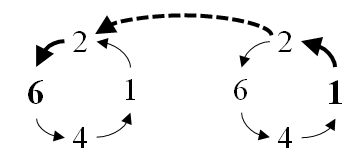
\includegraphics[width=2.in]{images/perm_square.png}
\caption{Diagram of $(1264)^2$, showing in particular how the permutation takes 1 to 6.}\label{fig:perm_square}
\end{center}
\end{figure}

\begin{enumerate}[(1)]
\item
Notice for all elements $x \neq 1, 2, 6, 4$, $x$ stays put in $(1264)$; hence $x$ stays put in $(1264)^2$.  So the product $(1264)^2$ does not involve any elements except $1, 2, 6$ and $4$.
\item
Now let's look at what happens when $x = 1, 2, 6,$ or $4$.   By squaring the cycle, we are applying it twice to each input; hence each input is moved two spots around the wheel (see Figure~\ref{fig:perm_square2}) .  In other words,  
\[
1 \to 6;  \quad 6 \to 1; \quad 2 \to 4; \quad 4 \to 2,
\]
Altogether: $(1264)^2 = (16)(24)$.
\end{enumerate}

\begin{figure}[ht]
\begin{center}
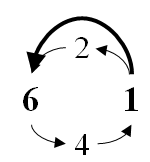
\includegraphics[width=0.8in]{images/perm_square2.png}
\caption{$(1264)^2$: streamlined notation}\label{fig:perm_square2}
\end{center}
\end{figure}


\end{example}

\noindent
With this methodology in mind, let's  explore powers of cycles a bit further.

\begin{exercise}\label{exercise:permute:4th_power}
Compute each of the following.
\begin{multicols}{3}
\begin{enumerate}[(a)]
\item
$(1 2 6 4)^3$
\item
$(1 2 6 4)^4$
\item
$(1 2 6 4)^5$
\end{enumerate}
\end{multicols}
\end{exercise}

\begin{exercise}\label{exercise:permute:6th_power}
Compute each of the following:
\begin{enumerate}[(a)]
\begin{multicols}{3}
\item
$(1 2 5 8 4 3)^2$
\item
$(1 2 5 8 4 3)^3$
\item
$(1 2 5 8 4 3)^4$
\item
$(1 2 5 8 4 3)^5$
\item
$(1 2 5 8 4 3)^6$
\item
$(1 2 5 8 4 3)^7$
\end{multicols}
\end{enumerate}
\end{exercise}

\noindent
Do you notice a pattern from these two exercises?  Let us investigate in a bit more detail: this will help us build up towards a proof of a general statement.

\begin{exercise}\label{exercise:permute:power of n-cycle1}
Let $X = \{1,2,\ldots,10\}$, let $A = \{2,5,7,8\}$, and let $\sigma \in S_X$ be the cycle  $\sigma = ( 2 5 7 8 )$. \begin{enumerate}[(a)]
\item
What is $\sigma(2)$? What is $\sigma^2(2)$? What is $\sigma^3(2)$? What is $\sigma^4(2)$ What is $\sigma^{3,482,991}(2)?$  
\item
What is $\sigma(5)$? What is $\sigma^2(5)$? What is $\sigma^3(5)$? What is $\sigma^4(5)$ What is $\sigma^{3,482,991}(5)?$  
\item
Fill in the blank: If $x \in A$ then $\sigma^k(x) = \sigma^{\bmod(k,\underline{~~}})$.
\item
What is $\sigma(1)$? What is $\sigma(3)$? 
\item
What general statement can you make about $\sigma^k(x)$ for $x \in X \backslash A$?
\item ** Let $K = \{k: \sigma^k(x) = x ~~\forall x \in X\}$. Is $2 \in K$?   Is $3 \in K$? Is $4 \in K$? Given any positive integer $k$, what's a simple way of telling whether or not $k \in K$?
\end{enumerate}
\end{exercise}

\noindent
Hopefully you're beginning to see the picture! To generalize these results, we need some additional terminology:

\begin{defn}
The \bfii{ order} of a cycle $\sigma$ is the smallest natural number $k$ such that $\sigma^k = {\var id}$.\index{Cycle!order of}\index{Order!of a cycle}   The order of $\sigma$ is denoted by the notation $|\sigma|$.
\footnote{This is in keeping with our practice of using $|\ldots|$ to denote the ``size'' of things.}
\end{defn}
After that long build-up, we now have (Ta-da!):

\begin{prop}\label{proposition:permute:order_of_cycle}
The order of a cycle is always equal to the cycle's length.
\end{prop}

%%% Removed (CPT)
%\begin{scratchwork}
%To prove this, we need to revisit cycle composition and look at it through the lens of function composition, rather than the procedure we learned.  Take $\mu = (1 2 6 4)$ from above as an example.  Let's look at what $\mu^4$ means element by element.
%\begin{itemize}
%\item
%For any element $x \neq 1, 2, 6, 4$, $\mu^4 (x) = \mu^3 (\mu(x)) = \mu^3 (x) =  \mu^2 (\mu(x)) = \mu^2 (x) = \mu(\mu(x)) = \mu(x) = x$
%\item
%For $x =1$:  $\mu^4 (1) = \mu^3 (\mu(1)) = \mu^3 (2) =  \mu^2 (\mu(2)) = \mu^2 (4) = \mu(\mu(4)) = \mu(6) = 1$
%\item
%Similarly then for $x = 2, 4, 6$:  $\mu^4(2) = 2$;  $\mu^4(4) = 4$; and $\mu^4(6) = 6$
%\end{itemize}

%Therefore for all elements $x$, $\mu^4(x) = x$.  And that is the definition of the identity permutation.  Hence $\mu^4 = {\var id}$.  For any one-cycle of length $n$ then, it makes sense, because for all elements that are not fixed, for all elements that are part of the cycle, we can think of that cycle as a circle with $n$ stops.  If you start anywhere on that circle, every time you compose by that cycle, you make one move around the circle.   So if you make $n$ moves around it, you will always end up where you began.  Formally then:
%\end{scratchwork}

\begin{proof}
To prove this, we essentially have to prove two things:
\begin{enumerate}[(A)]
\item
If $\sigma$ is a cycle of length $k$, then $\sigma^k = {\var id} $;
\item
If $\sigma$ is a cycle of length $k$, then $\sigma^j \neq {\var id} $~~$\forall j: 1 \le j < k.$
\end{enumerate}

\noindent
The proof for (A) follows the same lines as our investigations in Exercise~\ref{exercise:permute:power of n-cycle1}. In that exercise, we considered separately the elements of $X$ that are moved by the cycle, and those elements that are not moved by the cycle. 

\begin{exercise}\label{exercise:permute:length_equals_order} Prove part (A) by filling in the blanks.

\noindent
Let $\sigma \in S_X$ be an arbitrary cycle of length $k$.  Then $\sigma$ can be written as $ (a_1, a_2, \ldots a_k)$, for some set of elements $a_1, a_2, \ldots a_k$ in $X$.  In order to show that $\sigma^k = {\var id} $, it is sufficient to show that 
$\sigma^k(x) = \underline{~<1>~}  \forall x \in X$. 
Let $A$ be the set  $\{a_1, a_2, \ldots a_k\}$.  Now for any $x \in X$, there are two possibilities:  
\begin{enumerate}[(i)]
\item
$x \in  X \backslash A$;
\item
$x \in A$. 
\end{enumerate}

\noindent
We'll deal with these two cases separately (as we did  in Exercise~\ref{exercise:permute:power of n-cycle1}).

\begin{enumerate}[(i)]
\item
In this case, $\sigma(x) = \underline{~<2>~} $  It follows that $\sigma^2(x) = \sigma( \sigma(x)) = \sigma( \underline{~<3>~}) = \underline{~<4>~}$. We can use the same argument to show that $\sigma^3(x) = \underline{~<5>~}$, and that $\sigma^k(x) = \underline{~<6>~}$ for any natural number $\underline{~<7>~}$.
\item
In this case, then $x = a_j$ for some integer $j, 1 \le j \le \underline{~<8>~}$.  It follows from the definition of cycle that $\sigma(x) = \sigma(a_j) = \bmod(a_{j+1},k)$. Furthermore, $\sigma^2(x) = \sigma(a_{j+1}) = \underline{~<9>~}$. Similarly it follows that $\sigma^{k}(x) = a_{\bmod(j+ \underline{~<10>~},k)} = a_{\underline{~<11>~}} = x$.
\end{enumerate}

\noindent
Cases (i) and (ii) establish that  $\forall x \in X, \underline{~<12>~} = x$.  It follows that $\sigma^k = \underline{~<13>~}$.

\end{exercise}

\noindent
The proof of (B) is also structured as an exercise.

\begin{exercise}\label{exercise:permute:length_equals_order2}. In this exercise we use the same notation as part (A), that is: $\sigma \in S_X$ has length $k$ and is represented as: $\sigma = (a_1, a_2, \ldots a_k)$. 
\begin{enumerate}[(a)]
\item
What is $\sigma(a_1)$? What is $\sigma^2(a_1)$? What is $\sigma^3(a_1)$? What is $\sigma^{k-1}(a_1)$?
\item
Conclude from part (a) that  $\sigma^j \neq {\var id} $ for $j = 1,2,3, \ldots, k-1.$
\end{enumerate}
\end{exercise}
\end{proof}

\begin{example}\label{example:permute:cycle_order}
Here's a nice application of Proposition~\ref{proposition:permute:order_of_cycle}, which simply uses rules of function composition.  This should also give you a good start on the next exercise.
\[
(1 2 6 4)^6 = (1 2 6 4)^4 (1 2 6 4)^2 = {\var id} ~(1 6) (2 4) = (1 6)(2 4) \]
\end{example}

\begin{exercise}\label{exercise:permute:cycle_order_1}
Compute the following:
\begin{multicols}{2}
\begin{enumerate}[(a)]
\item
$(1 2 6 4)^{11}$
\item
$(1 2 5 8 4 3)^{53}$
\item
$(3 5 2)(1 3 6)(1254)^{102}$
\item
$(3 4 8) (4 5 6)^5 (1 3 2 5)^{10}$
\end{enumerate}
\end{multicols}
\end{exercise}

\subsection{Powers and orders of permutations in general}

Now that we know the order of cycles, let's see if we can tackle other permutations as well:

\begin{defn}
The \bfii{ order} of a permutation $\tau$ is the smallest positive integer $k$ such that $\tau^k = {\var id}$.\index{Order!of a permutation}   As before, the order of $\tau$ is denoted by the notation $|\tau|$. 
\end{defn}



\noindent
{\bf Proposition}: Let $\tau$ be a permutation, and let $k = |\tau|$. Then $\tau^{\ell} = {\var id}$ if and only if $\ell \equiv 0 \bmod{k}$.
\medskip

\begin{exercise}\label{exercise:permute:64}
Fill in the $\underline{~<\#>~}$ with the appropriate variables in the following proof of the proposition.
\hyperref[sec:permute:hints]{(*Hint*)}
\medskip

\noindent
{\bf Proof:} For any integer $\ell$ we may write $\ell = ak + b$, where $b \in \mathbb{Z}_{\underline{~<1>~}} $. It follows that
\[ \tau^{\ell} = \tau^{<\underline{2}> \cdot k + <\underline{3}>} = (\tau^{<\underline{4}> \cdot k})\tau^{<\underline{5}>} =   (\tau^k)^{<\underline{6}>}\tau^{<\underline{7}>} = ({\var id})^{<\underline{8}>}\tau^{<\underline{9}>} = \tau^{<\underline{10}>} . \]
Therefore $\tau^{\ell} = {\var id}$ if and only if $\tau^{<\underline{11}>} = {\var id}$. However, we know that $\underline{~<12>~} < k$, and we also know that $\underline{~<13>~}$ is the smallest positive integer such that  $\tau^{<\underline{14}>} = {\var id}$. Hence it must be the case that $b \equiv \underline{~<15>~} \bmod{k}$, which is the same thing as saying that  $\ell \equiv \underline{~<16>~} \bmod{\underline{~<17>~}}$.
\end{exercise}


Can we characterize the order of a permutation that is a product of disjoint cycles?  Let's explore.

\begin{example}\label{example:permute:disjoint_squared}
Let $\tau = (2 4)(1 6).$ Notice that $(2 4)$ and $(1 6)$ are disjoint, so they commute (recall Proposition~\ref{proposition:permute:disjoint_cycles_commute}). We also know that permutations are associative under composition. So we may compute $\tau^2$ as follows:

\noindent
$\tau^2 = {\large(} (2 4 )(1 6 ) {\large )} {\large(} (2 4 )(1 6 ) {\large )}$
 
~~~~=  $(2 4) {\large(} (1 6) (2 4 ) {\large )} (1 6 )$~~~~~~~~~~~(associative) 

~~~~=  $(2 4 ) {\large(} (2 4 ) (1 6)  {\large )} (1 6 )$~~~~~~~~~~~(commutative) 

~~~~=  ${\large(}  (2 4 ) (2 4 ) {\large )} {\large(}  (1 6) (1 6 ) {\large )}$~~~~~~~~~(associative) 

~~~~=  ${\var id}~{\var id}$ ~~~~~~~~~~~~~~~~~~~~~(2-cycles have order 2) 

~~~~=  ${\var id}$   

\end{example}


\begin{exercise}
\begin{enumerate}[(a)]
\item
Let $\sigma = (237)$ and $\tau = (458)$. By following the format of Example~\ref{example:permute:disjoint_squared}, show that $(\sigma \tau)^3 = {\var id} $ (write out each step, and cite the property used).
\item
** If $\sigma$ and $\tau$ are disjoint cycles with $|\sigma| = |\tau| = k$, what may you conclude about $| \sigma \tau |$? (You don't need to give a proof).
\end{enumerate}
\end{exercise}

\noindent
Associativity and commutativity are powerful tools for rearranging products of disjoint cycles, and bear in mind that any disjoint cycles commute.

\begin{exercise}\label{exercise:permute:k_power_disjoint_cycles}
\begin{enumerate}[(a)]
\item
Let $\sigma$ and $\tau$ be \emph{any} disjoint cycles. By following the format of Example~\ref{example:permute:disjoint_squared}, show that $(\sigma \tau)^2 = \sigma^2 \tau^2$ (write out each step, and cite the property used).
\item
If $\sigma$ and $\tau$ are disjoint cycles and $k$ is a natural number, what may you conclude about $(\sigma \tau)^k$? (You don't need to give a proof).
\end{enumerate}
\end{exercise}


% First we need a result.  By Proposition~\ref{proposition:permute:disjoint_is_simple}, we know disjoint cycles are commutative.  By the function composition, they are also associative.  Therefore if $\tau$ and $\sigma$ are two disjoint cycles, then 
% \[ (\tau \sigma)^n = (\tau \sigma)(\tau \sigma) \cdots (\tau \sigma) \mbox{ n times} = \tau^n \sigma^n \]
% \end{example}

%%Work in progress
\begin{figure}[htb]
	   \center{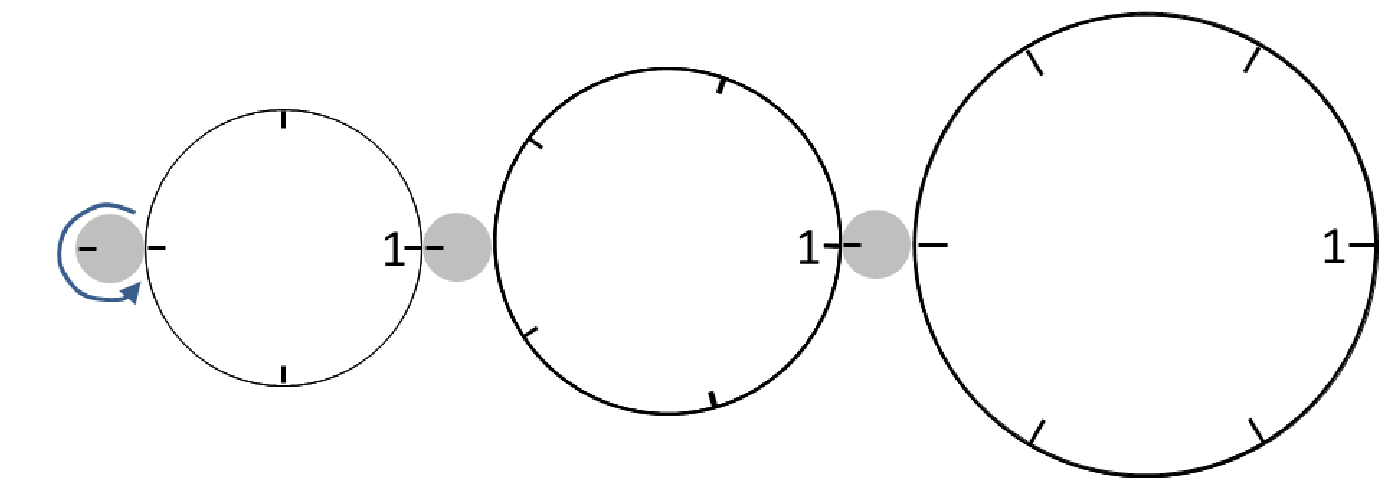
\includegraphics[width=3.5in]
	         {images/wheels1.png}}
	  \caption{\label{fig:wheels:2} How many times does the small gear(at left)  need to turn to return all gears to their original position? (Each turn rotates all  gears clockwise by 1 position.)}
\end{figure}
%Need text and example
\begin{exercise}\label{exercise:permute:disjoint_order_1}
Suppose then $\tau = (1 2 3)( 4 5)$. Compute each of the following
\begin{multicols}{3}
\begin{enumerate}[(a)]
\item 
$\tau^2$
\item 
$\tau^3$
\item 
$\tau^4$
\item 
$\tau^5$
\item 
$\tau^6$
\item
$\tau^7$
\end{enumerate}
\end{multicols}
\end{exercise}

\noindent
Notice what happened to the disjoint cycles in the previous exercise.  For instance $|(1 2 3)| = 3$, and in parts (a)-(e) of the exercise you had the repeating pattern $\{(1 3 2), {\var id}, (1 2 3), (1 3 2), {\var id}, \ldots\}$.  Similarly, the 2-cycle $(4 5)$ yielded the repeating pattern  $\{{\var id}, (4 5), {\var id}, (4 5) \ldots \}$.  

In $\tau^3, \tau^6, \tau^9, \ldots$  the $(1 2 3)^k$ part of $\tau^k$ becomes ${\var id} $,while in  $\tau^2, \tau^4, \tau^6, \ldots$ the $(4 5)^k$ part  becomes ${\var id} $.  In order for $\tau^k = {\var id} $, we must have both $(1 2 3)^k = {\var id} $ and $(4 5)^k = {\var id} $, which first happens when $k = 6$. It is no accident that $|(1 2 3)|$ and $|(4 5)|$ both divide 6. In fact,  we can prove  the following proposition.

\begin{prop}\label{proposition:permute:order_of_2disjoint_cycles}
If $\sigma$ and $\tau$ are disjoint cycles, then 

$$|\sigma \tau| = \mbox{ lcm }(|\sigma|,|\tau|),$$
where `lcm' denotes least common multiple.
\end{prop}

\begin{proof}  Let  $j \equiv |\sigma|, k \equiv |\tau|$, and $m \equiv \mbox{ lcm }(k,j)$. Then it's enough to prove:
\begin{enumerate}[(i)]
\item
$(\sigma \tau)^m = {\var id} $;
\item
$(\sigma \tau)^n \neq {\var id} $ if $n \in \mathbb{N}$ and $n < m$.
\end{enumerate}

\noindent
To prove (i), first note that $k$ divides $m$, so that $m = j \cdot p$ for some natural number $p$. Similarly, $m = k \cdot q$ for some $q \in \mathbb{N}$. It follows:

\noindent
$(\sigma \tau )^m = \sigma^m \tau^m$~~~~~(by Exercise~\ref{exercise:permute:k_power_disjoint_cycles})

~~~$=  \sigma^{j \cdot p} \tau^{ k \cdot q}$~~~~~(by definition of lcm)

~~~ $=  (\sigma^j)^p (\tau^ k)^q$~~~~~(by exponentiation rules)
\footnote{These are the same exponentiation rules you saw in high school algebra:  $x^{ab} = (x^a)^b$}

~~~$=   {\var id} ^p {\var id} ^q$~~~~~(by definition of order)

~~~$ = {\var id} $~~~~~(by definition of ${\var id} $).
\medskip

\noindent
To prove (ii), let $n < m$. It follows either $k$ or $j$ does \emph{not} divide $n$. Let's suppose it's $k$ (the case where it's $j$ is virtually identical). In this case we must have $n = p \cdot k + r$ where $p, $r$ \in \mathbb{N}$ and $r < k$. It follows:

\noindent
$(\sigma \tau )^n = \sigma^n \tau^n$~~~~~(by Exercise~\ref{exercise:permute:k_power_disjoint_cycles})

~~~$=  \sigma^{j \cdot p + r} \tau^n$~~~~~(substitution)

~~~ $=  (\sigma^j)^p \sigma^r \tau^n $~~~~~(by exponentiation rules)

~~~$=   {\var id} ^p \sigma^r \tau^n $~~~~~(by definition of order)

~~~$=   \sigma^r \tau^n $~~~~~~~~(by definition of identity)
\medskip

Now since $r < k$, and $|\sigma| = k$,  it follows that $\sigma^r \neq {\var id} $. Thus there is some $x$ such that $\sigma^r(x) \neq x$. But since $\sigma$ and $\tau$ are disjoint, it must be the case that $\tau(x) = x$. It follows that:
\medskip

$\sigma^r \tau^n (x) = \sigma^r (x) \neq x$. 
\medskip

\noindent
From this we may conclude that $(\sigma \tau )^n$ is \emph{not} the identity. This completes the proof of (ii).
\end{proof}\
\medskip

What Proposition~\ref{proposition:permute:order_of_2disjoint_cycles} establishes for two disjoint cycles is also true for multiple disjoint cycles. We state the proposition without proof, because it is similar to that of Proposition~\ref{proposition:permute:order_of_2disjoint_cycles} except with more details.\index{Disjoint cycles!powers of}

\begin{prop}\label{proposition:permute:order_of_disjoint}\index{Order!disjoint cycles}\index{Disjoint cycles!order of}
Suppose $\sigma_1, \sigma_2, \ldots , \sigma_n$ are $n$ disjoint cycles, where $k_1, k_2, \ldots, k_n$ are the lengths, respectively, of the $n$ disjoint cycles.  Then 
\[
|\sigma_1 \sigma_2  \cdots \sigma_n| = \mbox{ lcm }(k_1, k_2, \ldots, k_n). \]
\end{prop}

\noindent
Now we can find the order of any permutation by first representing it as a product of disjoint cycles.

\begin{exercise}\label{exercise:permute:Sn_orders}
What are all the possible orders for the permutations in each of the following sets (look back at your work for Exercise~\ref{exercise:permute:cycle_types}).
\begin{multicols}{3}
\begin{enumerate}[(a)]
\item
$S_6$
\item
$S_7$
\item
$S_8$
\end{enumerate}
\end{multicols}
\end{exercise}

\begin{exercise}\label{exercise:permute:disjoint_order_2}
Compute the following:
\begin{multicols}{2}
\begin{enumerate}[(a)]
\item
$| (1 2 5 4)^2 |$ 
\item
$| (1 3 6 5 8)^2 (4 7 3)^2 (1 2 5) |$
\item
$| (1 3 6 5 8)^{13} (1 2 5 4)^{11} (4 7 3) |$
\item
$| (1 2  3 4 5 6 7 8 9)^{300} |$
\end{enumerate}
\end{multicols}
\end{exercise}

\subsection{Transpositions and inverses}

%%\#\#\#\#\#\#\#\# Inverses should go earlier, after composition of cycles. There is no need to introduce inverses via transpositions, it is easiest to find the inverse of a cycle by example.

The simplest  nontrivial cycles are those of length 2. We will show that these 2-cycles are convenient ``building blocks'' which can be used to construct all other cycles. 

\begin{defn} \label{Transposition}
Cycles of length 2 are called  \bfii{ transpositions}\index{Transposition!definition of}.\index{Cycle!transposition}   We will often denote transpositions by the symbol $\tau$ (the greek letter ``tau'').
\end{defn}

\begin{exercise}\label{exercise:permute:example_transpositions}
Compute the following products:
\begin{enumerate}[(a)]
\begin{multicols}{2}
\item
$(1 4)(1 3) (1 2)$
\item
$(1 4)(1 8) (1 9)$
\item
$(1 6)(1 5) (1 4)(1 3)(1 2)$
\item
$(4 9)(4 8) (4 7)(4 6)(4 5)$
\item
$(1 2)(1 3)(1 4)(1 5) (1 6)(1 7)(1 8)$

\end{multicols}
\end{enumerate}
\end{exercise}

\begin{exercise}\label{exercise:permute:example_transpositions2}
In light of what you discovered in the previous exercise, write each cycle as a product of transpositions:
\begin{enumerate}[(a)]
\begin{multicols}{3}
\item
$(1 4 9 2)$
\item
$(1 2 3 4 5)$
\item
$(4 7 2 5 6 3)$
\item
$(a_1 a_2 a_3)$
\item
$(a_1 a_2 a_3 a_5 a_6)$
\item
$(a_1 a_2 a_3 a_5 a_6 a_7 a_8)$

\end{multicols}
\end{enumerate}
\end{exercise}

\noindent
The preceding exercises demonstrate the following proposition:

\begin{prop}\label{proposition:permute:transposition_formula}\index{Cycle!as products of transpositions}
Every cycle can be written as the product of transpositions:
\[ (a_1, a_2, \ldots, a_n ) = (a_1 a_n ) (a_1 a_{n-1} ) \cdots ( a_1 a_3 ) (a_1 a_2 ) \]
\end{prop}
\begin{proof}
The proof involves checking that left and right sides of the equation agree when they act on any $a_j$. We know that the cycle acting on $a_j$ gives $a_{j+1}$ (or $a_1$, if $j = n$); while the product of transpositions sends $a_j$ first to $a_1$, then to $a_{j+1}$.
\end{proof}

\noindent
Recall that we also know that any permutation can be written as a product of disjoint cycles, which leads to:

\begin{prop}
Any permutation of a finite set containing at least two elements can
be written as the product of transpositions. 
\end{prop}

\begin{proof} First write the permutation as a product of cycles: then write each cycle as a product of transpositions.
\end{proof}

\begin{exercise}\label{exercise:permute:prod_of_trans_1}
Express the following permutations as products of transpositions. 

\begin{enumerate}[(a)]
\begin{multicols}{2}
 \item
$( 1 4 3 5 6 )$
\item
$( 1 5 6 )( 2 3 4 )$
 \item
$( 1 4 2 6 )( 1 4 2 )$
 \item
$( 1 7 2 5 4 )( 1 4 2 3 )( 1 5 4 6 3 2 )$
 \item
$( 1 4 2 6 3 7 )(2 3 5 9)$
\item
$( 1 3 5 7 9 )(2 4 6 8 ) (1 9 7 5 3) (2 8 6 4)$
\end{multicols}
\end{enumerate}

\end{exercise}

\noindent
Even the identity permutation ${\var id}$ can be expressed as the product of transpositions:\index{Identity!of transpositions}

\begin{exercise}
Compute the following products:
\begin{enumerate}[(a)]
\begin{multicols}{3}
\item
$(1 2) (1 2)$
\item
$(5 7)(5 7)$
\item
$(a_1 a_2)(a_1 a_2)$
\end{multicols}
\item
What can you conclude about the inverse of a transposition?\index{Inverse!of transpositions}
\end{enumerate}
\end{exercise}

\noindent
The preceding exercise amounts to a proof of the following:

\begin{prop}\label{proposition:permute:trans_inv}
If $\tau$ is a transposition, $\tau^{-1} = \tau$.
\end{prop}

We can use the inverses of transpositions to build up the inverses of larger cycles:

\begin{prop}\label{proposition:permute:cycle_inv}
Suppose $\mu$ is a cycle: $\mu = (a_1 a_2 \ldots  a_n)$. Then $\mu^{-1} = (a_1 a_n a_{n-1}  \ldots a_2 )$.
\end{prop}

\begin{proof}
By Proposition~\ref{proposition:permute:transposition_formula} we can write 
\[ \mu = (a_1 a_n ) (a_1 a_{n-1} ) \cdots ( a_1 a_3) (a_1 a_2).
\]
Now consider first just the last two transpositions in this expression.
In the Functions chapter, we proved the formula  $(f \compose g)^{-1} = g^{-1} \compose f^{-1}$ for invertible functions $f$ and $g$.
Since transpositions are invertible functions, we have
\[
{\large(}(a_1 a_3)(a_1 a_2){\large)}^{-1} = (a_1 a_2)^{-1} ( a_1 a_3)^{-1} = (a_1 a_2 ) (a_1 a_3 ) \]
(the second equality follows because every transposition is its own inverse.)

If we apply similar reasoning to the last three transpositions in the expression, we find
\[
{\large(}(a_1 a_4)(a_1 a_3)(a_1 a_2){\large)}^{-1} = [(a_1 a_3)(a_1 a_2)]^{-1} ( a_1 a_4)^{-1} = (a_1 a_2 ) (a_1 a_3 ) (a_1 a_4) \]

 Applying this result inductively, we obtain finally: 
\[
\mu^{-1} = (a_1 a_2) ( a_1 a_3) \cdots (a_1 a_{n-1} ) (a_1 a_n ), \]
from this epression we may see that $a_1 \rightarrow a_n$, $a_n \rightarrow a_{n-1}, a_{n-1} \rightarrow a_{n-2}, \ldots, a_{2} \rightarrow a_{1}$, which 
corresponds to the cycle we want.
\end{proof}

We can now find the inverse of any product of cycles, by taking the inverses of the cycles in reverse order:\index{Inverse!of a cycle}\index{Cycle!inverse of}

\begin{example}
$\left[ ( 1 4 9 8 )( 2 4 6 8 ) \right] ^{-1} = ( 2 4 6 8 )^{-1}( 1 4 9 8 )^{-1} = ( 2 8 6 4 )(1 8 9 4) = ( 1 6 4)( 2 8 9)$. 
\end{example}

\begin{example}
$( 1 3 5 7) ^{-2} = \left[ ( 1 3 5 7 )^{-1} \right]^2 = ( 1 7  5 3 )^2 = ( 1 7 5 3 )(1 7 5 3) = ( 1 5 )(3 7)$. 
\end{example}


\begin{exercise}\label{exercise:permute:inv_comps}
Calculate each of the following.
\begin{multicols}{2}
\begin{enumerate}[(a)]    
\item
$(1 2 5 3 7)^{-1}$
 \item
$[(1 2)(3 4)(1 2)(4 7)]^{-1}$
\item
$[( 1 2 3 5 )( 4 6 7 )]^{-2}$
\item
$( 1 2 5 4 )^{-1} ( 1 2 3 )( 4 5 ) ( 1 2 5 4 )$
\item
$( 1 2 3 )( 4 5 ) ( 1 2 5 4 )^{-2}$
\item
$( 7 4 2 )^{-7} ( 2 8 6)^{-13}$

 \end{enumerate}
\end{multicols}
\end{exercise}

%\begin{example}\label{example:permute:transpositions_not_unique}
%Consider the permutation
%\[
%( 1 6 ) (2 5 3) = (1 6 )( 2 3 )( 2 5 ) 
%= (1 6 )( 4 5 )(2 3 )( 4 5 )(2 5 ).
%\]
%From this small example we can see there is no unique way to represent permutation as the
%product of transpositions. For instance, we can write the identity 
%permutation as $(1 2 )(1 2 )$, as $(1 3 )(2 4 )(1 3 )( 2 4 )$, and in
%many other ways. However, as it turns out, no permutation can be
%written as the product of both an even number of transpositions and an
%odd number of transpositions. For instance, we could represent the
%permutation $(1 6)$ by
%\[
%(2 3 )(1 6)( 2 3)
%\]
%or by
%\[
%(3 5) (1 6) (1 3) (1 6) (1 3) (3 5) (5 6).
%\]

\section{``Switchyard" and generators of the permutation group}
Switchyards are used by railroads to rearrange the order of train cars in a train (see Figure~\ref{fig:grandview}. In this section we will study a ``switchyard'' of sorts. The design of our mathematical ``switchyard'' is not realistic, but the example will help us understand some important fundamental properties of permutations.
\begin{figure}[ht]
\begin{center}
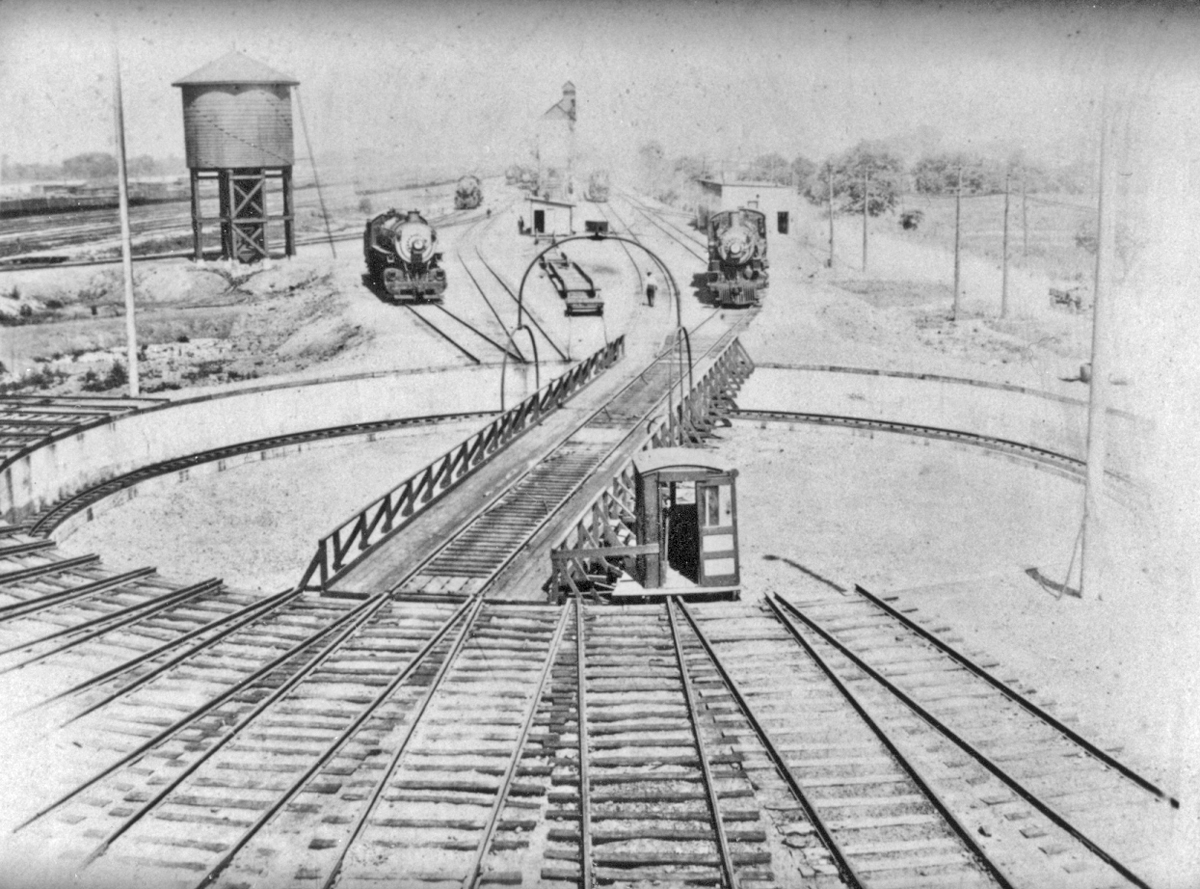
\includegraphics[width=4in]{images/GrandviewYard.jpg}
\caption{Grandview Yard (Pennsylvania Railorad) in Grandview Heights, OH around 1900 (source: \url{http://www.ghmchs.org/thisweek/photo-listing10.htm}. }\label{fig:grandview}
\end{center}
\end{figure}

Figure~\ref{fig:switchyard} shows how the switchyard works. The figure shows the particular case of a switchyard with 12 positions. A railroad train with 12 cars pulls in from the right, and circles around until it fills the circular track. 
\begin{figure}[ht]
\begin{center}
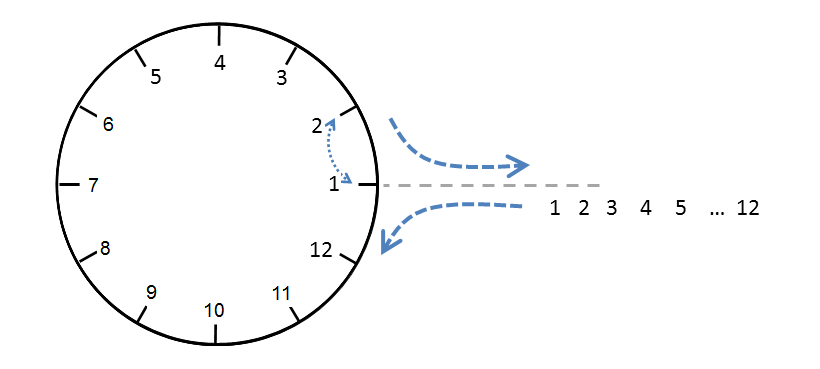
\includegraphics[width=4.5in]{images/switchyard.png}
\caption{``Switchyard'' diagram}\label{fig:switchyard}
\end{center}
\end{figure}

The positions (we'll call them \emph{slots} for short)  are numbered 1 through 12 as are the railroad cars. At the \emph{starting position}, each railroad car is at the corresponding numbered slot: car 1 is in slot 1, $\ldots$ car 12 is in slot 12.

From the starting position, the train can move in one of two ways:
\begin{itemize}
\item
The train can move circularly around the track, so that car 1 can end up at any one of the 12 slots. 
\item
Alternatively, the cars in slots 1 and 2 can switch places. 
\end{itemize}
These two types of motions can be represented as permutations. In tableau notation, the first row of the tableau corresponds to the train car, while the second row corresponds to the slot it moves to. For example, if the train cars $1,2,3, \ldots ,11, 12$ move counterclockwise one slot to occupy slots $2,3,4,\ldots ,12,1$ respectively, then the permutation (in tableau notation) is:
\[ \left( \begin{array}{cccccccccccc}
1 & 2 & 3 & 4 & 5 & 6 & 7 & 8 & 9 & 10 & 11 & 12 \\
2 & 3 & 4 & 5 & 6 & 7 & 8 & 9 & 10 & 11 & 12 & 1
 \end{array} \right)\] 
In cycle notation,  the same permutation would be $(1, 2, 3, 4, \ldots, 12)$, where we have put commas between cycle entries to distinguish the number 12 from consecutive 1 and 2.  We will denote this permutation by $r$. On the other hand, if cars 1 and 2 are switched, then this corresponds to the permutation $(1 2)$. We will denote this permutation by $t$.  In summary:
\[ r = (1,2,\ldots,12);\qquad  t = (1, 2).\]
Let's look at some other motions of the train. Suppose for example we shift the train counterclockwise by two positions. This corresponds to performing the permutation $r$ twice in succession, which is $r \compose r$ or $r^2$.   If we think about the process of composition, what's going on is the first $r$ moves car \#1 (which occupies slot \#1) to position \#2; while the second $r$ moves whatever's in slot 2 (which happens to be car \#1) to slot 3. The resulting composition can be interpreted as showing where each of the cars end up after both moves.  The same thing will be true  if we compose any number of permutations. 

It follows that all rearrangements of the cars that can be accomplished by the switchyard may be obtained as compositions of the permutations $r$ and $t$. So what rearrangements are possible? I'm glad you asked that question! The following exercises are designed to help you figure this out. But first, let's consider at one type of rearrangement that's particularly important. Suppose we want to switch two consecutive cars that are not 1 and 2: say for example we want to switch cars 5 and 6, and leave the rest of the cars unchanged.  Can we do this? 

At this point, in order to follow along the reader may find it helpful to make his/her own model of a switchyard.\footnote{The models in this section (and photos) were made by Holly Webb.} Figure~\ref{fig:switchyardHome} shows a simple model made out of a jar lid with numbers stuck on with putty.
\begin{figure}[ht]
\begin{center}
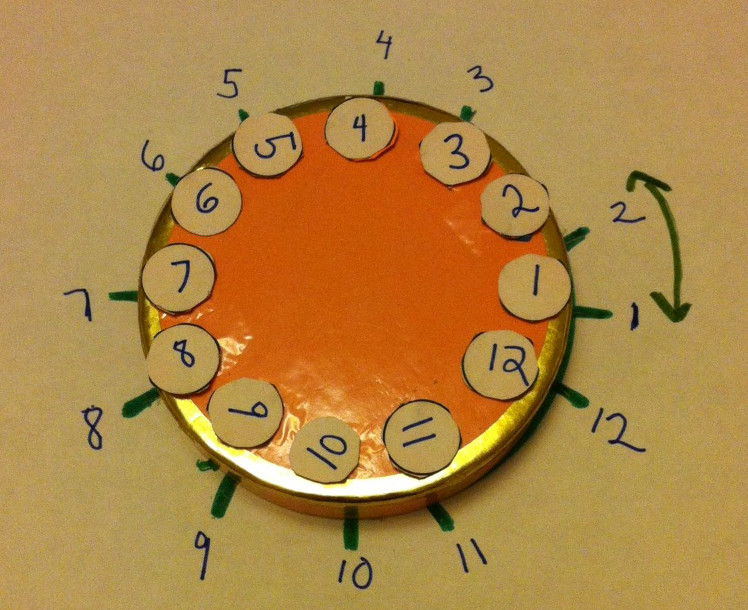
\includegraphics[width=2.5in]{images/switchyardHomeposition.jpg}
\caption{``Switchyard'' model in home position}\label{fig:switchyardHome}
\end{center}
\end{figure} 
We'll illustrate the motions necessary to switch cars  5 and 6  using the model.  First, we rotate cars 5 and 6 to slots 1 and 2 by rotating 4 slots clockwise. This permutation is shown in Figure~\ref{fig:switchyardCl4}, and is written mathematically as $r^{-4}$.
\begin{figure}[ht]
\begin{center}
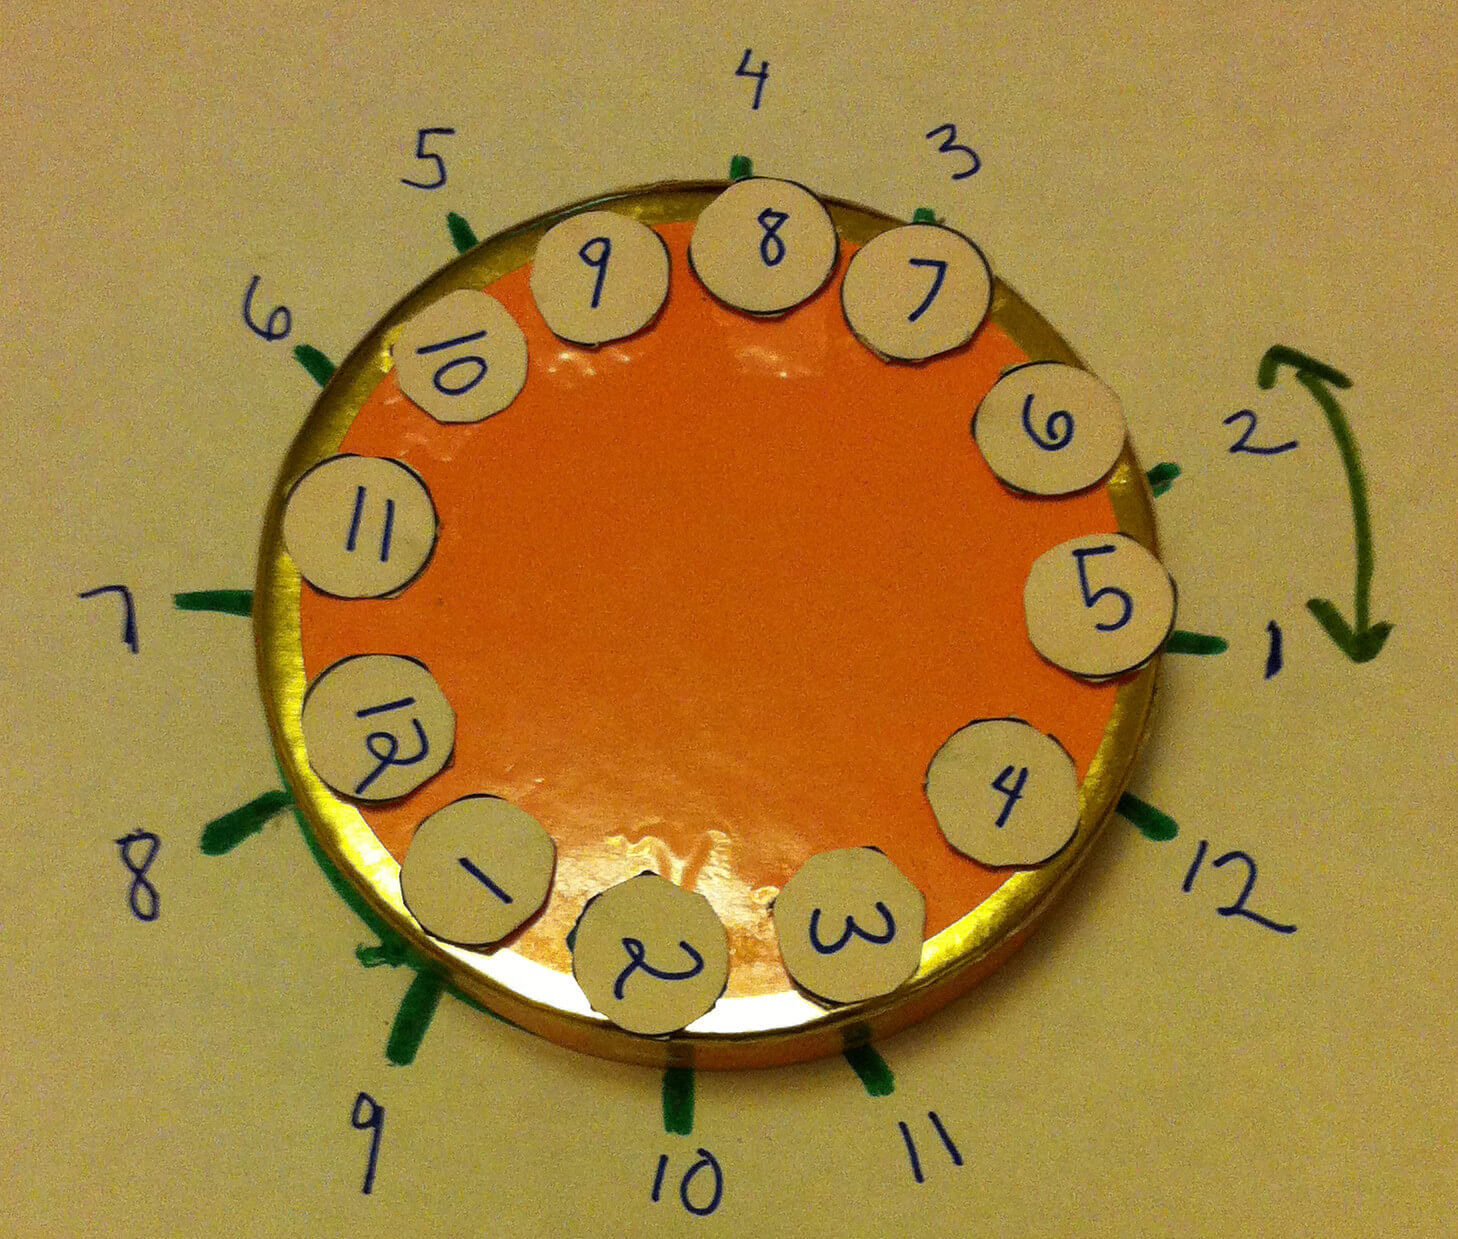
\includegraphics[width=2.5in]{images/switchyardCl4.jpg}
\caption{First stage in switching cars 5 and 6: clockwise rotation ($r^{-4}$.}\label{fig:switchyardCl4}
\end{center}
\end{figure} 

Next, we exchange the two cars (which we can do since they're in the first two positions). Figure~\ref{fig:switchyard_t} shows the switch, which is denoted by $t$.
\begin{figure}[ht]
\begin{center}
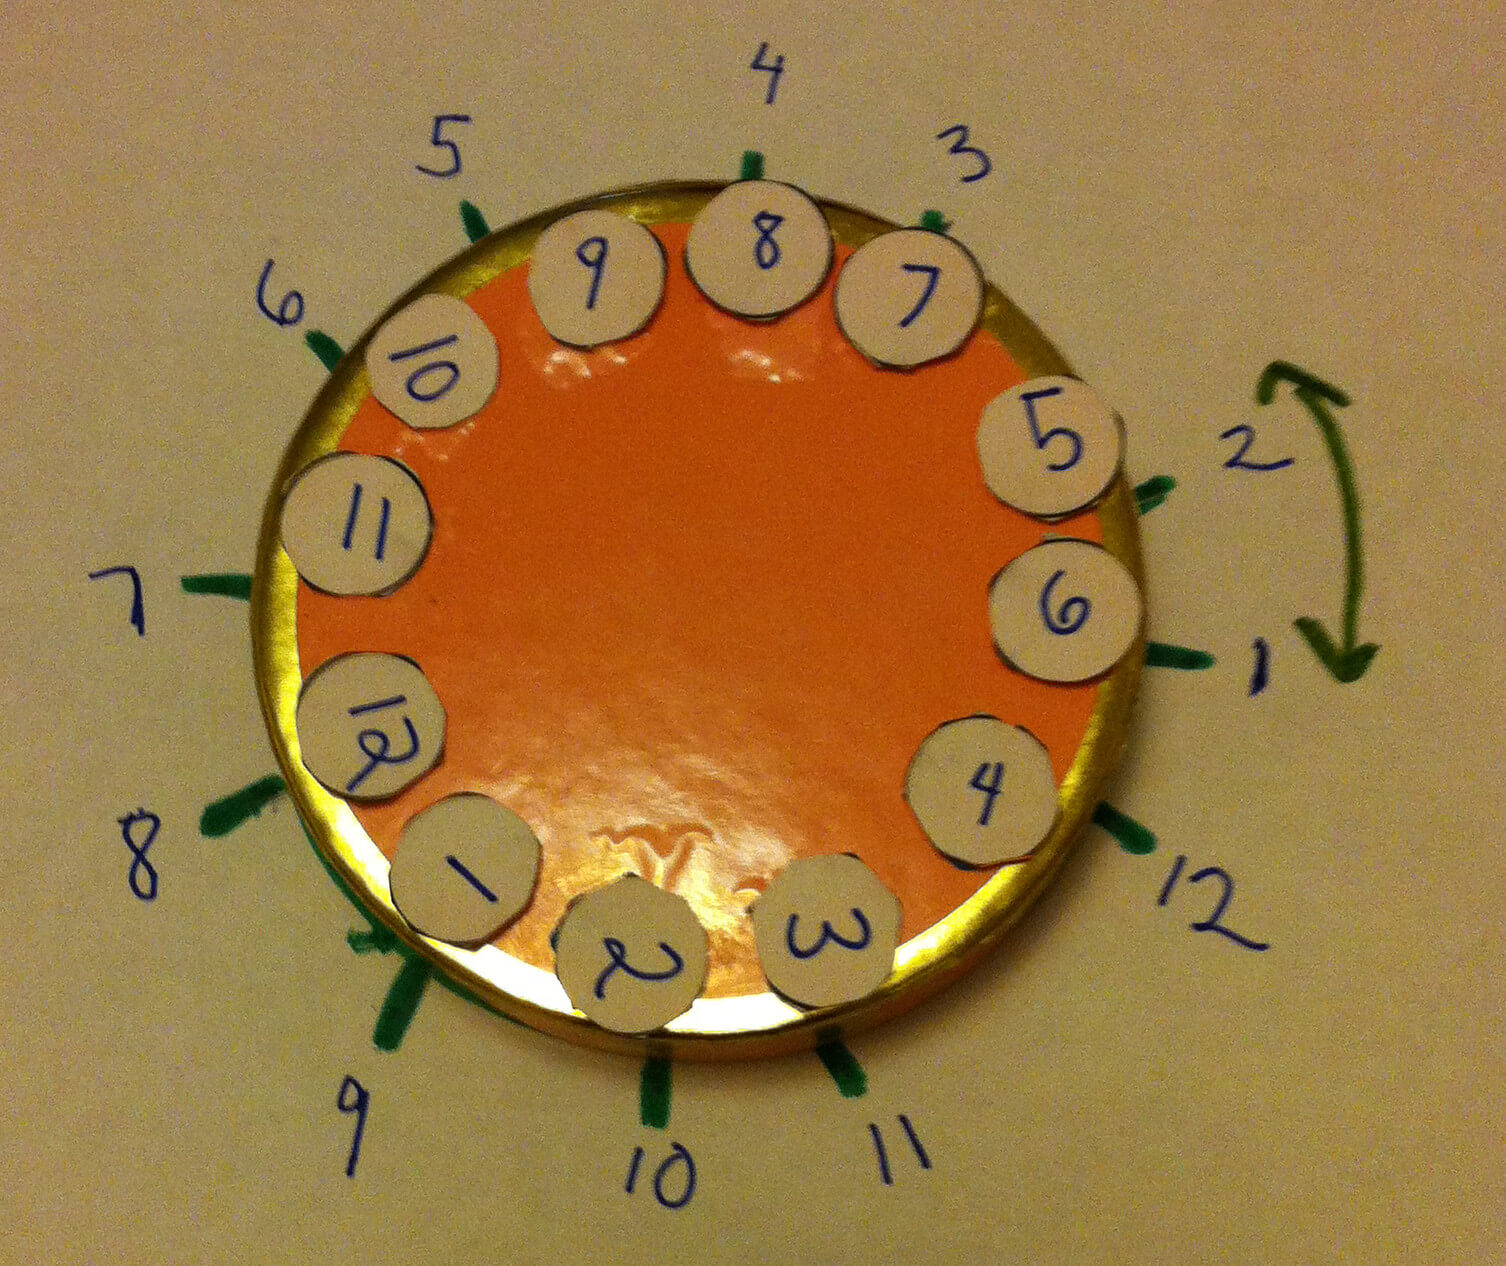
\includegraphics[width=2.5in]{images/switchyard_t.jpg}
\caption{Second stage in switching cars 5 and 6: switch ($t$).}\label{fig:switchyard_t}
\end{center}
\end{figure} 

Finally, all we need to do is rotate counterclockwise 4 slots ($r^4$), as shown in Figure~\ref{fig:switchyardCCL4}.
\begin{figure}[ht]
\begin{center}
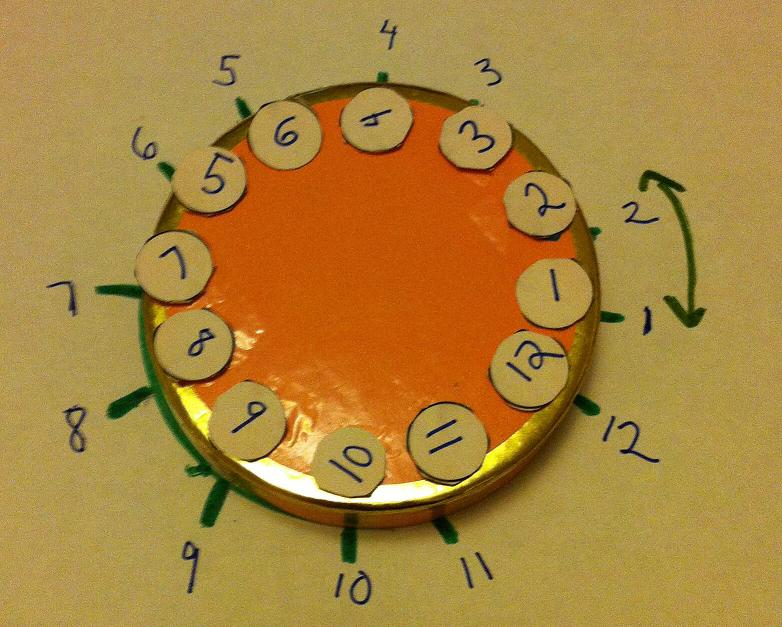
\includegraphics[width=2.5in]{images/switchyardCCL4.jpg}
\caption{Third stage in switching cars 5 and 6: counterclockwise rotation ($r^{4}$).}\label{fig:switchyardCCL4}
\end{center}
\end{figure} 

Altogether, these three steps give the composition $r^4 \compose t \compose r^{-4}$ (remember that permutations are applied right to left, just like functions).  Note also that in the case of a 12-slot switchyard, $r^{-4}$ could also be written $r^8$, since a clockwise rotation of 4 slots is the same as a counterclockwise rotation of 8 slots.  (If the switchyard has $n$ positions, the general rule is that $r^{-m} = r^{n-m}$, as we saw in the Symmetries chapter.)

\begin{exercise}\label{exercise:permute:switchyard1}
First we'll look at a switchyard with 4 positions.  As above, $r$ = counterclockwise rotation by 1 position = $(1, 2, 3, 4)$; while $t$  exchanges two cars: $t = (1,2)$. 
\begin{enumerate}[(a)]
\item
Write $(2,3)$, $(3,4)$, and $(4,1)$ as products of powers of $r$ and $t$. (Together with (12), these are all the  consecutive 2-cycles.)
\item
Write $(1,2,3)$, $(2,3,4)$, $(3,4,1)$, $(4,1,2)$ as products of powers of $r$ and $t$. (These are all the counterclockwise consecutive  3-cycles.)
\item
Write $(1,3,2)$, $(2,4,3)$, $(3,1,4)$, $(4,2,1)$ as products of powers of $r$ and $t$. (These are all the clockwise consecutive 3-cycles.)
\hyperref[sec:permute:hints]{(*Hint*)}
\item
Write $(1,3)$ as products of powers of $r$ and $t$.
\item
Show that any transposition can be written as products of powers of $r$ and $t$.
\item
Show that any permutation  on 4 elements (that is, any permutation in $S_4$) can be obtained as a product of powers of $r$ and $t$).
\end{enumerate}
\end{exercise}

\begin{exercise}\label{exercise:permute:switchyard2}
Now we'll look at a general switchyard with $n$ positions. In this case, rotation by 1 position is given by  $r= (1,2,\ldots,n)$. We  use the same transposition, $t = (1,2)$.
\begin{enumerate}[(a)]
\item
Write the transposition $(k,k\oplus 1)$ as a product of powers of $r$ and $t$. Here $\oplus$ denotes addition mod $n$.
\item
Show that any consecutive cycle $(m,m\oplus 1,\ldots,m \oplus  p )$ can be written as a product of powers of $r$ and $t$ by filling in the blanks:

\begin{itemize}
\item
First, $(m,m \oplus 1,\ldots,m \oplus  p )$ can be written as a product of consecutive transpositions as \_\_\_\_\_\_\_\_\_\_\_\_\_\_\_\_.
\item
Then, by replacing each transposition in this expression with its expression in terms of  products of \_\_\_\_\_\_\_\_\_\_\_\_\_\_\_\_, then we obtain an expression for \_\_\_\_\_\_\_\_\_\_\_\_\_\_\_\_ as a product of \_\_\_\_\_\_\_\_\_\_\_\_\_\_\_\_.
\end{itemize}

\item
Write the transposition $(1,k)$ as a product of a cycle of length $k$ and a cycle of length $k-1$. 
\item
Prove that any transposition $(1,k)$ can be written as a product of consecutive transpositions.
\item
Prove that any transposition $(1,k)$ can be written as a product of powers of $r$ and $t$.
\item
Prove that any transposition $(p,q)$ can be written as a product of powers of $r$ and $t$.
\item
Prove that any permutation in $S_n$ can be obtained as a product of powers of $r$ and $t$.
\end{enumerate}
\end{exercise}
What we have shown in the previous exercise is that the two permutations $r$ and $t$ \emph{generate} the group $S_n$. In other words, all of the information contained in the huge and complicated group $S_n$ is characterized in just two permutations! The study of group generators is an important part of group theory, but unfortunately it is beyond the level of this course.  


\section{Other groups of permutations}
\subsection{Even and odd permutations}

We saw in the previous section that any permutation can be represented as a product of transpositions. However, this representation is not unique. Consider for instance:
\begin{itemize}
\item
${\var id}  = (1 2) ( 1 2)$
\item
${\var id}  = (1 3 )(2 4 )(1 3 )( 2 4 )$
\item
${\var id}  = (1 5 )(2 6 )(7 9 )( 1 4 )(3 4)(3 4)(1 4)(7 9)(2 6)(1 5)$
\end{itemize}

\noindent
Although these representations of ${\var id} $ are vastly different, by some ``strange coincidence'' they all involve the product of an even number of 
transpositions.  

%It turns out that this is generally true. We will not prove this here,\footnote{A proof-by-exploration is given in the supplementary materials} but since we will need this fact we will state it as a proposition.
%
%\begin{prop}\label{proposition:permute:EvenIdentity} Suppose $\tau_1, \tau_2, \ldots, \tau_n$ are transpositions such that $\tau_1 \tau_2\cdots \tau_n
%= {\var id}$. Then $n$ must be even.
%\end{prop}
%
%
%
%%%% Should leverage permutation matrices
%%%% Also can prove by induction on the number of elements being permuted. Move the transposition involving (n) to the far left. Process results in # transpositions differ by even. 
\begin{exercise}
***** Write ${\var id} $ as a product of an odd number of transpositions (If you succeed, you automatically get an $A$ in this course!)
\end{exercise}

As you might guess from the previous exercise, there's something fishy going on here. 
To get to the bottom of this, we need to  get a better handle on what happens when you multiply a permutation by a transposition. 
In particular, we know that any permutation can be written as a product of  disjoint cycles: so what happens to these cycles when we multiply by a transposition? To get warmed up, let's first look at some special cases.

\begin{exercise}
Write $\tau \sigma$  as the products of disjoint cycles, where $\sigma = (12345678)$ and:
$(a)~\tau= (25);~~ (b)~\tau= (16);~~ (c)~\tau=(48) ;~~ (d)~\tau=(35)$.
\end{exercise}


As always it is helpful to have a good representation of the situation, preferably in pictures. For the following argument, we will represent a cycle as a ``pearl necklace'', as shown in Figure~\ref{fig:pearl}. This is not so different from our previous representation of cycles (for instance, in Figure~\ref{fig:cycle}), but we are not including labels for the particular elements in the cycle because we want to emphasize the general structure and not get bogged down in details. 

\begin{figure}[ht]
\begin{center}
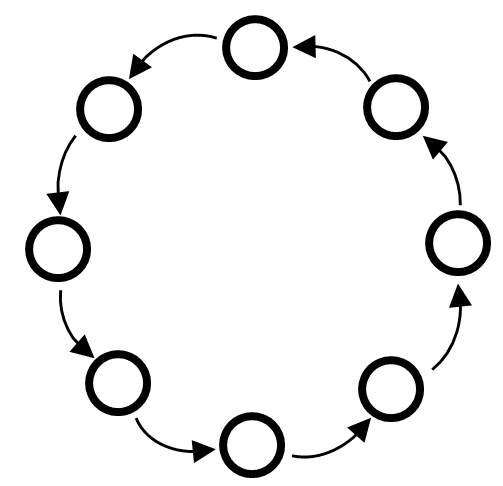
\includegraphics[width=1.5in]{images/pearl_necklace.png}
\caption{``Pearl necklace'' representation of a cycle.}\label{fig:pearl}
\end{center}
\end{figure}


Figure~\ref{fig:abC} shows how we may represent the multiplication $(ab)C$ of transposition $(ab)$ with cycle $C$, where $a$ and $b$ are elements included within $C$. The transposition effectively redirects the arrow pointing into $a$, so that now it points into $b$. The transposition also redirects the arrow pointing into $b$ so that it now points into $a$. As a result, there are now two cycles instead of one. The sum of the lengths of the two cycles is equal to the length of the original cycle.

\begin{figure}[ht]
\begin{center}
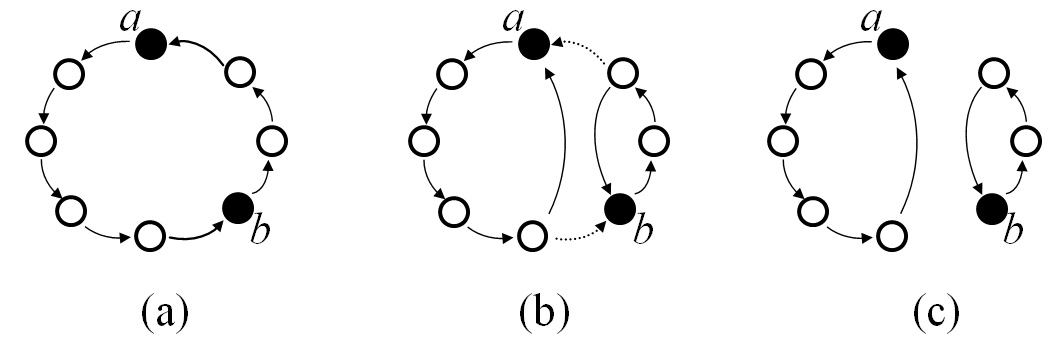
\includegraphics[width=4in]{images/(ab)C.png}
\caption{(a) Cycle $C$, including elements $a$ and $b$;~ (b) Product of transposition $(ab)$ with cycle $C$, showing redirection of arrows into $a$ and $b$;~ (c) The result of $(ab)C$ is two separate cycles.}\label{fig:abC}
\end{center}
\end{figure}

Using this representation, we can now investigate what happens when we multiply a transposition $(ab)$ times an \emph{arbitrary} permutation $P$. We already know that $P$ can be thought of as a collection of disjoint cycles (plus stationary  elements, that are unaffected by $P$). There are several possibilities for how $a$ and $b$ can fit within the cycles of $P$, as shown in Figure~\ref{fig:abC2}.  Each possibility may or may not change the number of cycles, as well as the sum of the lengths of all cycles.   

\begin{figure}[ht]
\begin{center}
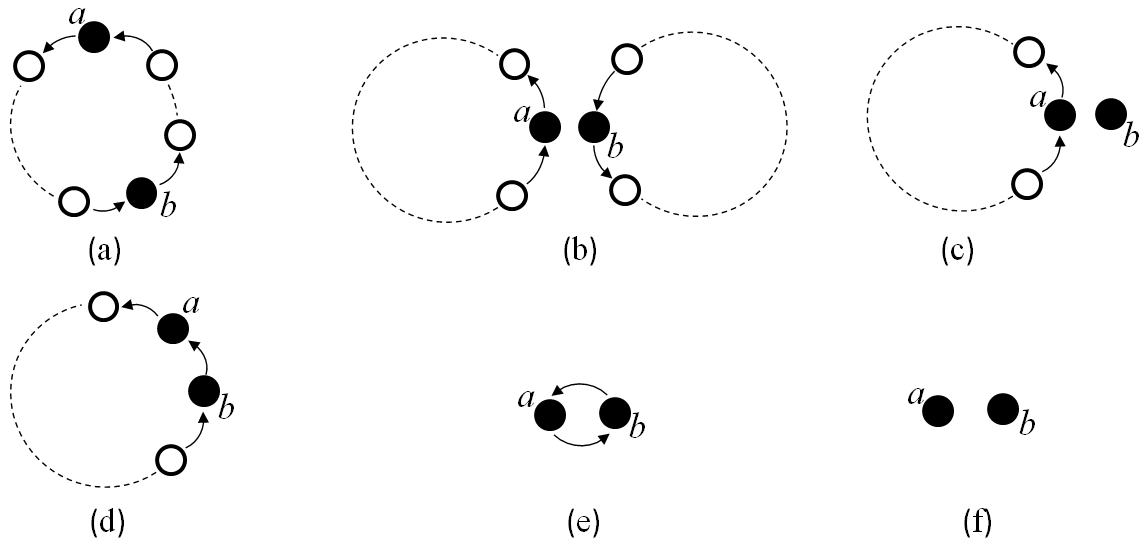
\includegraphics[width=5in]{images/(ab)C2.png}
\caption{Multiplication of $(ab)$ times a permutation $P$, showing the different ways that $a$ and $b$ can fit within the cycles (and stationary elements)  of $P$. Note that  case (a) corresponds to the situation described in Figure~\ref{fig:abC}.) }\label{fig:abC2}
\end{center}
\end{figure}


\begin{exercise}
Draw a picture (similar to Figure~\ref{fig:abC}(c)) for each of the possibilities (a)--(f) in Figure~\ref{fig:abC2} showing the effect of the transposition $(ab)$ on the cycles.   Keep in mind that the transposition merely redirects the arrows into $a$ and $b$ so that they point into $b$ and $a$, respectively.
\end{exercise}

\begin{exercise}
Using your results from the previous exercise, complete Table~\ref{transposition_table}.
\end{exercise}

\begin{table}[!htb]
\caption{Multiplication of permutation by transpositions}\label{transposition_table}
\begin{tabular}{|p{1.9cm}|p{2.9cm}|p{2.9cm}|p{3.5cm}|}
\hline 
\rule{0pt}{2.6ex} Diagram in Figure~\ref{fig:abC2}&  Change in number of cycles ($\Delta_{\text{cyc}}$)   & Change in sum of cycle lengths ($\Delta_{\text{sum}}$) & $(\Delta_{\text{cyc}}-\Delta_{\text{sum}}) (\bmod{2})$  \rule[-1.2ex]{0pt}{0pt} \tabularnewline
\hline
\hline 
\rule{0pt}{2.6ex} (a)  &  +1  & 0  & 1 \rule[-1.2ex]{0pt}{0pt} \tabularnewline
\hline 
\rule{0pt}{2.6ex} (b)  &  \_\_\_\_\_ & \_\_\_\_\_ & \_\_\_\_\_ \rule[-1.2ex]{0pt}{0pt} \tabularnewline
\hline 
\rule{0pt}{2.6ex} (c)  &  \_\_\_\_\_ & \_\_\_\_\_  & \_\_\_\_\_ \rule[-1.2ex]{0pt}{0pt} \tabularnewline
\hline 
\rule{0pt}{2.6ex} (d)  &  \_\_\_\_\_ & \_\_\_\_\_  & \_\_\_\_\_ \rule[-1.2ex]{0pt}{0pt} \tabularnewline
\hline 
\rule{0pt}{2.6ex} (e)  & $-1$ & $-2$ & \_\_\_\_\_ \rule[-1.2ex]{0pt}{0pt} \tabularnewline
\hline 
\rule{0pt}{2.6ex} (f)  &  \_\_\_\_\_ & \_\_\_\_\_ & \_\_\_\_\_  \rule[-1.2ex]{0pt}{0pt} \tabularnewline
\hline 
\end{tabular}
\end{table}


If you did the previous exercise correctly, you will find that no matter where the transposition falls,  the column entry under ``$(\Delta_{\text{cyc}}-\Delta_{\text{sum}}) \bmod{2}$"  is always 1. This motivates the following definition:

\begin{defn} for any permutation $P$, the number (sum of cycle lengths -- number of cycles) mod 2 is called the \bfii{ parity} of $P$.\index{Permutation!parity} A permutation with parity 0 is called an \bfii{ even permutation}, while a  permutation with parity 1 is called an \bfii{ odd permutation}. \index{Permutation!odd and even}.  Often books will use the terms ``even parity'' and ``odd parity''  instead of parity 0 and 1, respectively.
\end{defn}
\noindent
Note that the disjoint sets of even and odd permutations of $n$ objects form a \emph{partition} of the set $S_n$. As we saw in the equivalence relations chapter, this means that we can define an equivalence relation such that all permutations with the same parity are equivalent.

Using this new terminology  we may summarize our findings from Table~\ref{transposition_table} as follows. Every time I multiply a permutation by a transposition, I change the parity. So if I multiply together an even number of transpositions, the parity is 0; while if I multiply together an odd number of transpoitions, the parity is 1. 

Now here's the punch line. We know that \emph{every} permutation can be written as a product of transpositions. 
From what we have just shown, an odd permutation must be the product of an odd number of transpositions; while an even permutation must be the product of an even number of transpositions. It is \emph{impossible} to write an even permutation as the product of an odd number of transpositions; and vice versa. 
We summarize our conclusions in the following theorem.

\begin{prop}\label{proposition:permute:even_and_odd}
A permutation $P$ can be written as the product of an even number of transpositions if and only if $P$ is an even permutation. 
Also,  $P$ can be written as the product of an odd number of transpositions if and only if $P$ is an odd permutation. 
\end{prop}


\begin{exercise}
Prove that it is impossible to write the identity permutation as the product of an odd number of cycles.
\end{exercise}



%
%If a given permutation is the product of an even number of transpositions, then (sum of 
%Don't worry, we'll get to the bottom of this: but first, some definitions.
%
%%So how you represent a permutation as a product of transpositions \emph{is not} unique; but the whether those representations of the permutation always have an even or odd number of transpositions \emph{is} unique.  This fact leads to the following proposition and defintions.
%
%\begin{defn} If a permutation $\sigma$ can be expressed as the product of an even
%number of transpositions, then  we call $\sigma$ an \bfii{ even permutation}. \index{Permutation!even}\index{Even permutation}
%Similarly, if $\sigma$ can be expressed as the product of an odd
%number of transpositions, then  we call $\sigma$ an \bfii{ odd permutation}. \index{Permutation!odd}\index{Odd permutation}
%\end{defn}
%
%At this point we don't know anything about even or odd permutations. It's conceivable  for instance, that there might be permutations that are both even and odd. Is this actually possible? Let's find out! We begin by investigating the products of transpositions and cycles.
%
%\begin{exercise}
%Compute the following products:
%\begin{enumerate}[(a)]
%\begin{multicols}{2}
%\item
%( 3 4)(2 3 4 5 6 7)
%\item
%( 2 7)(2 3 4 5 6 7)
%\item
%(2  5)(2 3 4 5 6 7)
%\item
%( 3 7)(2 3 4 5 6 7)
%\end{multicols}
%\end{enumerate}
%\end{exercise}
%
%We want to develop a general formula for the product of a transposition $(a_i a_j)$ and a cycle $(a_1 a_2 \ldots a_n)$. In light of the previous exercise, it appears there are three cases to consider:
%
%\begin{enumerate}[(i)]
%\item
%$ j = i+1$;
%\item
%$\{i,j\} = \{1,n\}$
%\item
%$ j \ne i+1$ and $\{i,j\} \ne \{1,n\}$
%\end{enumerate}
%
%We will investigate case (iii), and leave cases (i) and (ii) as exercises. In case (iii) then, let $\sigma = (a_i a_j)(a_1 a_2 \ldots a_n)$. It follows that 
%\begin{align*}
%\sigma( a_1 ) & = a_2 \\
%              & \vdots   \\
%\sigma( a_{i-1} ) & = a_j \\
%\sigma( a_{j} ) & = a_{j+1}\\
%              & \vdots   \\
%\sigma( a_{n}) & = a_1.
%\end{align*}
%
%\noindent
%which implies that $\sigma$ contains the cycle:  $(a_1 a_2 \ldots a_{i-1} a_j \ldots a_n)$. But there is \emph{another} cycle as well:
%\begin{align*}
%\sigma( a_i ) & = a_{i+1} \\
%              & \vdots   \\
%\sigma( a_{j-1} ) & = a_i 
%\end{align*}
%
%\noindent
%In summary:  
%\[
%(a_i a_j)(a_1 a_2 \ldots a_n) = (a_1 a_2 \ldots a_{i-1} a_j \ldots a_n)(a_i a_{i+1} \ldots a_{j-1})
%\]
%
%\noindent
%We have thus re-expressed $\sigma$ as the product of disjoint cycles. Let us compare the left- and right-hand sides of this equation:
%
%\begin{itemize}
%\item
%The left-hand side has two cycles; the right-hand side also has two cycles.
%\item 
%The sum of cycle lengths on the left-hand side is $2 + n$; the sum of cycle lengths on the right-hand side is $(n - j + i) + (i - j) = n$.
%\item
%If we take the sum of cycle lengths minus the number of cycles, the left-hand side gives $(n+2)-2=n$ and the right-hand side gives $n-2$. What's important to note here is that these two numbers differ by an \emph{even} number.
%\end{itemize}
%
%The following exercises look at cases (i) and (ii):
%
%\begin{exercise} \emph{(Case (i))}
%
%\begin{enumerate}[(a)]
%\item
%Give a general formula for $(a_i a_{i+1})(a_1 a_2 \ldots a_n)$, where $1 \le i \le n$.
%\item
%How many cycles are on the left-hand side of your formula? How many disjoint cycles on the right-hand side?
%\item
%What is the sum of the lengths of cycles on the left-hand side of your formula? The right-hand side?
%\item
%What is the (sum of the lengths of cycles) -- (number of cycles)  on the left-hand side of your formula? The right-hand side? Do these two numbers differ by an even number?
%\end{enumerate}
%\end{exercise}
%
%\begin{exercise} \emph{(Case (ii))}
%
%\begin{enumerate}[(a)]
%\item
%Give a general formula for $(a_1 a_n)(a_1 a_2 \ldots a_n)$.
%\item
%How many cycles are on the left-hand side of your formula? How many disjoint cycles on the right-hand side?
%\item
%What is the sum of the lengths of cycles on the left-hand side of your formula? The right-hand side?
%\item
%What is the (sum of the lengths of cycles) -- (number of cycles)  on the left-hand side of your formula? The right-hand side? Do these two numbers differ by an even number?
%\end{enumerate}
%\end{exercise}
%
%\noindent
%To recap: so far we have (sum of the lengths of cycles) -- ($\#$ cycles) always changes by an even number.
%\medskip
%
%But there are other possibilities for multiplying a 2-cycle with an $n$-cycle. It's also possible that the 2-cycle elements are not all contained in the $n$-cycle: that is, we can have a product $(a_j b)(a_1 a_2 \ldots a_n)$ where $b \neq a_k \forall k$.
%
%\begin{exercise} \emph{(2-cycle not contained)}
%
%\begin{enumerate}[(a)]
%\item
%Give a general formula for $(a_j b)(a_1 a_2 \ldots a_n)$, where $b \neq a_k \forall k$.
%\item
%How many cycles are on the left-hand side of your formula? How many disjoint cycles on the right-hand side?
%\item
%What is the sum of the lengths of cycles on the left-hand side of your formula? The right-hand side?
%\item
%What is the (sum of the lengths of cycles) -- (number of cycles)  on the left-hand side of your formula? The right-hand side? Do these two numbers differ by an even number?
%\end{enumerate}
%\end{exercise}
%
%\noindent
%There is one additional possibility we need to consider. Suppose we have two disjoint cycles, and we multiply on the left by a 2-cycle that intersects both cycles. That is, suppose we have the product 
%$(a_i b_j)(a_1 a_2 \ldots a_n)(b_1 b_2 \ldots b_m)$:
%
%\begin{exercise} \emph{(2-cycle with two disjoint cycles)}
%\begin{enumerate}[(a)]
%\item
%Give a general formula for $(a_i b_j)(a_1 a_2 \ldots a_n)(b_1 b_2 \ldots b_m)$.
%\item
%How many cycles are on the left-hand side of your formula? How many disjoint cycles on the right-hand side?
%\item
%What is the sum of the lengths of cycles on the left-hand side of your formula? The right-hand side?
%\item
%What is the (sum of the lengths of cycles) -- (number of cycles)  on the left-hand side of your formula? The right-hand side? Do these two numbers differ by an even number?
%\end{enumerate}
%\end{exercise}
%
%\noindent
%All of the preceding investigations lead us to the following result.
%
%
%We can leverage Proposition~\ref{proposition:permute:EvenIdentity} to prove something similar for permutations in general.
%
%\begin{prop}\label{proposition:permute:even_and_odd}
%Suppose the permutation $\sigma$ can be expressed as the product of transpositions in two different ways, that is:
%\[ \sigma = \tau_1 \cdots \tau_n \quad \text{and} \quad \sigma = \tau_1' \cdots \tau_m'. \]
%Then either $n$ and $m$ are both even, or $n$ and $m$ are both odd (another way of saying this is that $n+m$ is always even).
%\end{prop}
%
%\begin{proof}
%We may equate the two given expressions for $\sigma$ to obtain: 
%\[\tau_1 \cdots \tau_n  = \tau_1' \cdots \tau_m'.\]
% Multiplying both sides of this equation on the left by $\tau_n \cdots \tau_1$ and using the fact that $\tau_j \tau_j = {\var id}$, we obtain
%\[ {\var id} = \tau_n \cdots \tau_1 \cdot \tau_1' \cdots \tau_m'.\]
%By Proposition~\ref{proposition:permute:EvenIdentity}, it follows that $n+m$ is even. 
%\end{proof}
%
%From Proposition~\ref{proposition:permute:even_and_odd} we may deduce that there are two types of permutations, depending on whether it takes an even or odd number of transpositions to express the permutation. We formalize this distinction in the following definition.
% 
%\begin{defn} If a permutation $\sigma$ can be expressed as the product of an even
%number of transpositions, then  we call $\sigma$ an \bfii{ even permutation}. \index{Permutation!even}\index{Even permutation}
%Similarly, if $\sigma$ can be expressed as the product of an odd
%number of transpositions, then  we call $\sigma$ an \bfii{ odd permutation}. \index{Permutation!odd}\index{Odd permutation}. The property of ``evenness'' or ``oddness'' is called \bfii{ parity}\index{Permutation!parity} (so we will say that an even permutation has even parity, and similarly for odd).
%\end{defn}

\begin{exercise}
Suppose $P$ is an $n$-cycle.  How can you tell  whether $P$ is an even or odd permutation?
\end{exercise}


In the following exercises you will explore a bit further the parity properties of permutations. 

\begin{exercise}\label{exercise:permute:Ex95}\label{ex:evenoddprod} %%% Note for some reason the conventional label doesn't work
\begin{enumerate}[(a)]
\item
Prove that the product of two even permutations is even.
\item
Prove that the product of two odd permutations is even.
\item
What is the parity of  the product of an even permutation and an odd permutation?  What about the product of an odd permutation and an even permutation? \emph{Prove} your answers.
%\item 
%Given that $\sigma$ and $\mu$ are cycles, prove that $\sigma \mu$ is even if and only if 
%$|\sigma| +  |\mu| - 2$ is even.
%\item \label{Prod2Perm}
%Given that $\sigma, \mu, and \rho$ are cycles, prove that $\sigma \mu \rho$ is even if and only if 
%$|\sigma| +  |\mu| + |\rho| - 3$ is even.
%\item \label{Prod3Perm}
%Can you generalize the results of (\ref{Prod2Perm}) and  (\ref{Prod2Perm}) to products of an arbitrary number of cycles?
\end{enumerate}
\end{exercise}
%
%
%Following the previous exercise, we may derive a rule for determining the parity of a permutation from its cycle structure.
%
%\begin{prop}\label{proposition:permute:EvenOddDisjoint}
%Suppose that the permutation $\sigma$ can be written as the product of disjoint cycles as
%\[\sigma = \sigma_1 \sigma_2 \cdots \sigma_N. \]
%Then $\sigma$ is even if and only if 
%$|\sigma_1|+ |\sigma_2| +  \ldots + |\sigma_N| - N$ is even.
%\end{prop}
%Note that we can ``even'' with ``odd'' in Proposition~\ref{proposition:permute:EvenOddDisjoint} and the result is still true.
%
%\begin{exercise}
%Fill in the blanks to complete the following  proof of Proposition~\ref{proposition:permute:EvenOddDisjoint}.
%
%\noindent
%From Proposition~$\_\_\_\_\_$, we know that any cycle $\sigma_j$ can be written as the product of $\_\_\_\_\_\_\_\_$ transpositions. Putting these products together, It follows that the product of the cycles $\sigma_1, \sigma_2, \ldots \sigma_n$ can be written as the product of $(\_\_\_\_\_\_) + (\_\_\_\_\_\_) + \ldots + (\_\_\_\_\_\_\_)$ transpositions, which can be rearranged to obtain $\_\_\_\_\_\_\_\_\_\_\_\_\_\_\_\_\_\_\_$. It follows from Proposition~$\_\_\_\_\_\_\_\_$ that this quantity is even if and only if $\_\_\_\_\_\_\_\_$ is even, which gives us the result.
%\end{exercise}

% \begin{itemize}
% \item
% The number of transpositions is even  if $\sum_{j=1 \dots J} |\sigma_j| - J$ is even;\index{Transpositions!number of}
% \item
% The number of transpositions is odd  if $\sum_{j=1 \dots J} |\sigma_j| - J$ is odd.
% \end{itemize}
% Here $\{ \sigma_1, \ldots, \sigma_J \}$ denote the cycles in $\sigma$'s disjoint cycle representation: $\sigma = \sigma_1 \sigma_2 \cdots \sigma_J$.
% \end{prop}

% \begin{proof}
% Suppose that the transpositions in the product are $\tau_1, \tau_2, \ldots, \tau_N$, so that $\tau_1 \tau_2 \cdots \tau_N = \sigma$. Since permutations are associative,
% we can multiply the $\tau_j$'s any order we want: so let's start multiplying from the right.

% \begin{itemize}
% \item
% Take first $\tau_{N-1} \tau_N = \mu_2$. On the left-hand side of this equation we have a transposition times a 2-cycle: so (sum of lengths of cycles) -- ($\#$ of cycles) = $4 - 2 = 2$.  If we rewrite $\mu_2$ as a product of disjoint cycles, it follows that   (sum of lengths of cycles in $\mu_2$) -- ($\#$ of cycles in $\mu_2$)  must be even.
% \item
% Now take $\tau{N-2} \mu_2 = \mu_3$. We've just seen that (sum of lengths of cycles in $\mu_2$) -- ($\#$ of cycles in  $\mu_2$) is even. Since $|\tau_{N-2}|=2$, then including  $\tau_{N-2}$ increases the sum of lengths by 2 while increasing the number of cycles by 1, making a net change of $2-1 = 1$.  If we write $\mu_3$ as a product of disjoint cycles, it follows that
  % (sum of lengths of cycles in $\mu_3$) -- ($\#$ of cycles in $\mu_3$)  must be odd.
% \item
% We may repeat this process a total of $N-1$ times. At the final stage, we will have $\tau_1 \mu_{N-1} = \mu_{N}$, where $\mu_{N}$ represents $\sigma$ as  a product of disjoint cycles: $\mu_{N} = \sigma_1 \sigma_2 \cdots \sigma_J$. If $N$ is even, then $\sum_{j=1 \dots J} |\sigma_j| - J$ is even; and if  $N$ is odd, then $\sum_{j=1 \dots J} |\sigma_j| - J$ is odd.
% \end{itemize}
% \end{proof}

% %, then any other product of transpositions
% %equaling $\sigma$ must also contain an even number of transpositions.  In this case we call $\sigma$ an \bfii{ even permutation}.

% %\bigskip{}
% %Similarly, if $\sigma$ can be expressed as the product of an odd
% %number of transpositions, then any other product of transpositions
% %equaling $\sigma$ must also contain an odd number of transpositions.  In this case we call $\sigma$ an \bfii{ odd permutation}. 
% %\end{prop}
% %
% %To prove this, we first need a fact that we will assume without proof, because of the complexity of the proof.
% %
% %\begin{notation}{id_even}
% %If the identity is written as the product of $r$ transpositions,
% %\[
% %id = \tau_1 \tau_2 \cdots \tau_r,
% %\]
% %then $r$ is an even number.  In other words, the identity permutation is even.
% %\end{notation}
% %
% %Now on to our proof of the above proposition, which is actually easy and quite clever.  We will prove even, you will prove odd.
% %
% %\begin{proof}
% %Suppose that we have the permutation $\sigma$ and it can be represented in the following two ways.
% %\[
% %\sigma = \sigma_1 \sigma_2 \cdots \sigma_m = \tau_1 \tau_2 \cdots
% %\tau_n, 
% %\]
% %where $m$ is even. We must show that $n$ is also an even number.  The
% %inverse of $\sigma^{-1}$ is $\sigma_m \cdots \sigma_1$. Now, 
% %\[
% %{\var id} = \sigma \sigma_m \cdots \sigma_1
% %= \tau_1  \cdots \tau_n \sigma_m \cdots \sigma_1,
% %\]
% %Since the identity is an even permutation and $m$ is even, then $n$ must be even.  
% %
% %The proof for the case in which $\sigma$ can be expressed as an odd number of transpositions is left
% %as the next exercise.  
% %\end{proof}
% %
% %\begin{exercise}\label{exercise:permute:odd_is_odd}
% %If $\sigma$ can be expressed as an odd number of transpositions, show
% %that any other product of transpositions equaling $\sigma$ must also
% %be odd. 
% %\end{exercise}

\begin{exercise}\label{exercise:permute:Sn_even_odd}
For each of the following sets, describe which permutations are even and which are odd, according to their cycle structure.
\hyperref[sec:permute:hints]{(*Hint*)}
\begin{multicols}{3}
\begin{enumerate}[(a)]
\item
$S_6$
\item
$S_7$
\item
$S_8$
\end{enumerate}
\end{multicols}
\end{exercise}

\subsection{The alternating group}\label{sec:AlternatingGroup}

We have shown that all permutations are either even or odd. In other words, for any $n \in \mathbb{Z}$ we have that $S_n$ is the union of two disjoint sets: $S_n = A_n \cup B_n$, where $A_n$ and $B_n$ are the even and odd permutations respectively.

\begin{exercise}\label{exercise:permute:S_nequiv}
Use the sets $A_n$ and $B_n$ to define an equivalence relation on $S_n$, and verify that it is an equivalence relation.
\hyperref[sec:permute:hints]{(*Hint*)}
\end{exercise}

We are particularly interested in the set $A_n$, because it has nice properties with respect to permutation product:

\begin{exercise}\label{exercise:permute:A_nGroupProps}
\begin{enumerate}[(a)]
\item
Show that ${\var id}  \in A_n$.
\item
Show that if $\sigma \in A_n$, then $\sigma^{-1} \in A_n$.
\hyperref[sec:permute:hints]{(*Hint*)}
\item
Show that if $\sigma, \mu \in A_n$, then $\sigma \mu \in A_n$. 
\hyperref[sec:permute:hints]{(*Hint*)}
\end{enumerate}
\end{exercise}

In light of the previous exercise, it's beginning to look like $A_n$ could be a group under permutation product. Let's check off the group properties:
\begin{itemize}
\item Is $A_n$ closed under permutation product? Yes, according to Ex.~\ref{exercise:permute:A_nGroupProps}(c).
\item Does $A_n$ have an identity element? Yes, according to Ex.~\ref{exercise:permute:A_nGroupProps}(a).
\item Does $A_n$ have inverses for every element? Yes, according to Ex.~\ref{exercise:permute:A_nGroupProps}(b).
\item Is $A_n$ associative? Yes, because the operation is composition, and composition is associative.
\end{itemize}

\noindent
We have thus essentially proven the following proposition:

\begin{prop}\label{proposition:permute:An_group}
The set $A_n$ is a group. 
\end{prop}


\begin{defn} \label{Alternating_Group}
The group $A_n$\label{alternatinggroup} of even permutations is called the \bfii{
alternating group on $n$ letters}\index{Group!alternating}. 
\end{defn}

\begin{exercise}
Prove or disprove: the set of odd permutations $B_n$ is also a group.
\end{exercise}

%Let's prove $A_n$ is actually a permutation group.  From the last exercise we can imagine gathering all of the even permutations of $S_n$ into a set.  Hence we can see the set $A_n \subset S_n$.  What else do we need to do to prove the set $A_n$ is a permutation group?  Prove that it's a group.
% 
% 
%\begin{proof}
%\begin{itemize}
%\item
%Since permutations are functions, $A_n$ is associative under composition.
%\item
%Given two even permutations $\tau$ and $\mu$, we know each permutation is represented by an even number of transpositions.  Hence the composition of the two can be represented by all the transpositions from each permutation %lined up in their corresponding order.   Hence $\tau \mu$ and $\mu \tau$ must also be even permutations.  Hence $A_n$ is closed. 
%\item
% The identity is an even permutation and
%therefore is in $A_n$. 
%\item
%If $\sigma$ is an even permutation, then
%\[
%\sigma = \sigma_1 \sigma_2 \cdots \sigma_r,
%\]
%where $\sigma_i$ is a transposition and $r$ is even. Since the inverse
%of any transposition is itself, 
%\[
%\sigma^{-1} = \sigma_r \sigma_{r-1} \cdots \sigma_1
%\]
%is also in $A_n$.
%\end{itemize}
%\end{proof}
% 
 
We know that $A_n$ is a group -- but how big is it? Of course, it depends on the number of odd permutations $B_n$, since $A_n$ and $B_n$ together make up $S_n$.
So which is bigger: $A_n$ or $B_n$? The answer is \ldots neither!

\begin{prop}\label{proposition:permute:Alternating1}
The number of even permutations in $S_n$, $n \geq 2$, is equal to the
number of odd permutations; hence, $| A_n | = n!/2$.
\end{prop}
 
 \begin{proof}
The key to the proof is showing that there is a \emph{bijection} between $A_n$  and $B_n$. Since a bijection is one-to-one and onto, this means that $A_n$ and $B_n$ must have
exactly the same number of elements.

To construct a bijection, notice that $(1 2) \in S_n$ and define a function $f: A_n \rightarrow S_n$ by: $f(\sigma) = (1 2) \compose \sigma$. (Notice that we are taking $A_n$ as our domain, and not $S_n$).
To show that $f$ is a bijection, we need to show three things:
\begin{enumerate}[(a)]
\item
$B_n$ is a valid codomain for $f$: that is, $f(\sigma) \in B_n ~\forall \sigma \in A_n$;
\item
$f:A_n \rightarrow B_n$ is onto: that is, $\forall \mu \in B_n ~\exists \sigma \in A_n$ such that $f(\sigma) = \mu$;
 \item
$f$ is one-to-one: that is, $f(\sigma_1) = f(\sigma_2)$ implies $\sigma_1 = \sigma_2$.
\end{enumerate}

Parts (a) -- (c) will be proven by (none other than) you, in the following exercise:

\begin{exercise}\label{exercise:permute:prove}
\begin{enumerate}[(a)]
\item
Show part (a).  
\hyperref[sec:permute:hints]{(*Hint*)}
\item
Show part (b). 
\hyperref[sec:permute:hints]{(*Hint*)}
\item
Show part (c). 
\hyperref[sec:permute:hints]{(*Hint*)}
\end{enumerate}
\end{exercise}

\end{proof}
%first choose any transposition $\tau$ in $S_n$ ince $n \geq 2$, such a
%$\sigma$ exists.  Define
%\[
%\lambda_{\sigma} : A_n \rightarrow B_n
%\]
%by
%\[
%\lambda_{\sigma} ( \tau ) = \sigma  \tau .
%\]
%Suppose that $\lambda_{\sigma} ( \tau ) = \lambda_{\sigma} ( \mu )$.
%Then $\sigma  \tau = \sigma  \mu$ and so 
%\[
%\tau = \sigma^{-1} \sigma \tau = \sigma^{-1} \sigma \mu =
%\mu.
%\]
%Therefore, $\lambda_{\sigma}$ is one-to-one.  We will leave the proof
%that $\lambda_{\sigma}$ is surjective to the reader.
%\end{proof}
 
\begin{exercise}\label{exercise:permute:A4}
\begin{enumerate}[(a)]
\item 
What is $| A_4 |$?
\item
List all the permutations of $A_4$ (Write them in cycle notation. Make sure you have them all -- you should have as many as part (a) indicates).
\end{enumerate}
\end{exercise}

\begin{exercise}\label{exercise:permute:A6_A7_A8}
Give all possible cycle structures for elements in each of the following sets.
\begin{enumerate}[(a)]
\begin{multicols}{3}
\item
$A_6$
\item
$A_7$
\item
$A_8$
\end{multicols}
\end{enumerate}
\end{exercise}


\markright{EXERCISES}
\section{Additional exercises}
\exrule
 
 
 
{\small
\begin{enumerate}
 
  
\item \label{ex:permute:Ad1}
Show that $A_{10}$ contains an element of order 15.
\hyperref[sec:permute:hints]{(*Hint*)}
 
 
\item
Does $A_8$ contain an element of order 26?
 
 
\item %7
Find an element of largest order in $S_n$ for $n = 3, \ldots, 10$. 
 
  
 \item
In Chapter \ref{complex} we used the term `non-abelian' to describe groups in which not all elements commute. To show that a group is non-abelian, it's enough to find a single pair of elements $a, b \in S_n$ which do not commute (that is, $ab \neq ba$).
\begin{enumerate}[(a)]
\item
Prove that $S_n$ is non-abelian for $n \geq 3$. 
\item
Show that $A_n$ is non-abelian for $n \geq 4$.
\item
Prove that $D_n$ is non-abelian for $n \geq 3$.
 \end{enumerate} 

\item
Let $\sigma$ be a permutation in $S_n$.  
\begin{enumerate}[(a)]
\item
Show that there exists an integer $k>1$ such that $sigma^k = \sigma$.
\item
Show that there exists an integer $\ell>1$ such that $sigma^{\ell} = \sigma^{-1}$.
\item
Let $K$ be the set of \emph{all} integers $k>1$ such that $sigma^k = \sigma$. Show that $K$ is an infinite set (that is, $K$ has an infinite number of elements).
\item
Let $L$ be the set of \emph{all} integers $\ell>1$ such that $sigma^{\ell} = \sigma^{-1}$. Show that $L$ is an infinite set.
\item
What is the relationship between the sets $K$ and $L$?
\end{enumerate}


\item \label{ex:permute:Ad2}
Let $\sigma \in S_n$. Prove that $\sigma$ can be written as the
product of at most $n-1$ transpositions.
\hyperref[sec:permute:hints]{(*Hint*)}

\item \label{ex:permute:Ad3}
Let $\sigma \in S_n$. If $\sigma$ is not a cycle, prove that $\sigma$
can be written as the product of at most $n-2$ transpositions.
\hyperref[sec:permute:hints]{(*Hint*)}

\item \label{ex:permute:Ad4}
If $\sigma$ is a cycle of odd length, prove that $\sigma^2$ is also a
cycle.
\hyperref[sec:permute:hints]{(*Hint*)}  
  
\item
Prove that in $A_n$ with $n \geq 3$, any permutation is a product of
cycles of length~3.  
  
\item
Using ``switchyard'', we proved that $S_n$ is generated by the permutations $(12)$ and $(12 \ldots n)$.
Prove that the group $S_n$ is generated by
the following sets of permutations.
\begin{enumerate}
 
 \item
$(1 2), (13), \ldots, (1n)$
 
 \item
$(1 2), (23), \ldots, (n- 1,n)$
 
 
\end{enumerate}
 
 
\item
Let $G$ be a group and define a function $f_g : G \rightarrow G$ by
$f_g(a) = g a$.  Prove that $f_g$ is a permutation of $G$.
 
 
 \item
Let $\tau = (a_1, a_2, \ldots, a_k)$ be a cycle of length $k$.
\begin{enumerate}
 
 \item
Prove that if $\sigma$ is any permutation, then
\[
\sigma \tau \sigma^{-1 } = ( \sigma(a_1), \sigma(a_2), \ldots,
\sigma(a_k))
\]
is a cycle of length $k$.
 
 \item
Let $\mu$ be a cycle of length $k$. Prove that there is a permutation
$\sigma$ such that $\sigma \tau \sigma^{-1 } = \mu$.
 
\end{enumerate}
 
 
\item
For $\alpha$ and $\beta$ in $S_n$, define $\alpha \sim \beta$ if there
exists an $\sigma \in S_n$ such that $\sigma \alpha \sigma^{-1} =
\beta$.  Show that $\sim$ is an equivalence relation on $S_n$.
 
 
\item
Let $\sigma \in S_X$. If $\sigma^n(x) = y$, we will say that $x \sim
y$. 
\begin{enumerate}
 
 \item
Show that $\sim$ is an equivalence relation on $X$.
 
 \item
If $\sigma \in A_n$ and $\tau \in S_n$, show that $\tau^{-1} \sigma
\tau \in A_n$. 
 
\item
Define the \bfii{ orbit}\index{Orbit} of $x \in X$ under the permutation $\sigma \in
S_X$ to be the set 
\[
{\cal O}_{x, \sigma} = \{ y : x \sim y  \}.
\]
Compute the orbits of $\alpha, \beta, \gamma$ where
\begin{align*}
\alpha & = (1254) \\
\beta & = (123)(45)\\
\gamma & = (13)(25).
\end{align*}
 
 \item
If ${\cal O}_{x, \sigma} \cap {\cal O}_{y, \sigma} \neq \emptyset$,
prove that ${\cal O}_{x, \sigma} = {\cal O}_{y, \sigma}$.  The orbits
under a permutation $\sigma$ are the equivalence classes corresponding
to the equivalence relation $\sim$.
 
 
\item
A subgroup $H$ of $S_X$ is \bfii{
transitive}\index{Subgroup!transitive} if for every $x, y \in X$, 
there exists a $\sigma \in H$ such that $\sigma(x) =y$. Prove that
$\langle \sigma \rangle$ is transitive if and only if ${\cal O}_{x,
\sigma} = X$ for some $x \in X$. 
 
 
\end{enumerate}
 
 
\item
Show that  $\alpha^{-1} \beta^{-1} \alpha \beta$ is even for all $\alpha,
\beta \in S_n$. 
 
\end{enumerate}
}